\documentclass[a4paper,11pt]{article}
\usepackage{geometry}
 \geometry{
 a4paper,
 total={170mm,257mm},
 left=20mm,
 top=20mm,
 }

 \usepackage{multirow}
\usepackage{colortbl}
 \usepackage{hhline}

 \usepackage{lipsum}  %%% Lorem ipsum

\setlength{\headheight}{30.0pt}
\setlength{\footskip}{20pt}


\usepackage{hyperref}
\hypersetup{
    colorlinks=True,
    linkcolor={blue!20!black},
    filecolor=magenta,      
    urlcolor=cyan,
}



 \usepackage[export]{adjustbox}
\usepackage[english]{babel}
\usepackage[utf8]{inputenc}
\usepackage{fancyhdr}
\usepackage{multicol}

\pagestyle{fancy}
\fancyhf{}
\rhead{\textit{Pul074BEX004}}
\lhead{\textit{Amrit Prasad Phuyal}}
\rfoot{\thepage}


\usepackage{mathpazo} % Palatino font
\usepackage{graphicx}
\usepackage{float}

%%%% Anser environment use %%%% Anser environment use %%%% Anser environment use \input{./AnsENV.tex}
%% use \begin{A... {**** argument***}
\RequirePackage{scrextend}

\newenvironment{A}[1]{\textit{Answer:}{\begin{addmargin}[2em]{2em}{#1}\end{addmargin} 
  }}

% just leave some space   
%% use \begin{A... {**** argument***}
\RequirePackage{scrextend}

\newenvironment{A}[1]{\textit{Answer:}{\begin{addmargin}[2em]{2em}{#1}\end{addmargin} 
  }}

% just leave some space   
%% use \begin{A... {**** argument***}
\RequirePackage{scrextend}

\newenvironment{A}[1]{\textit{Answer:}{\begin{addmargin}[2em]{2em}{#1}\end{addmargin} 
  }}

% just leave some space    %% Answer environment 

%%% Question Environment%%%  use 
%%% Question Environment%%%  use 
%%% Question Environment%%%  use \input{./QueENV.tex}   to include
%% Use \begin{Q}....\end{Q}

\newcounter{QC}
\setcounter{QC}{1}
\newenvironment{Q}[1]{
    \section{Question -\arabic{QC}} \stepcounter{QC}{\large\textbf{#1}}
}

%%% Question Environment%%%

   to include
%% Use \begin{Q}....\end{Q}

\newcounter{QC}
\setcounter{QC}{1}
\newenvironment{Q}[1]{
    \section{Question -\arabic{QC}} \stepcounter{QC}{\large\textbf{#1}}
}

%%% Question Environment%%%

   to include
%% Use \begin{Q}....\end{Q}

\newcounter{QC}
\setcounter{QC}{1}
\newenvironment{Q}[1]{
    \section{Question -\arabic{QC}} \stepcounter{QC}{\large\textbf{#1}}
}

%%% Question Environment%%%

 %% Question Environment 
%%%%%% include  Titles.%%%% use \input{./CP}%%%
%%%use """"""""    \CP{}{}{}{}   """" %%%% and 4 argument to craete Title page 
%%%%%%%%%%%%%%%%%%%%%%%%%%%%%%%%%%%%%%%%%%%%%%%%%%%%%%%%%%%%%%%%%
%%%argument number
%% 1=major header ## Course name 
%% 2=minor4 heading ## lab/assignmet no
%% 3=Title  ## Assignment or Lab title
%% 4=submitted to::## input receiver Name"
%%%%%%%%%%%%%%%%%%%%%%%%%%%%%%%%%%%%%%%%%%%%%%%%%%%%%%%%%%%%%%%%%


\usepackage{mathpazo} % Palatino font
\usepackage{graphicx}
\usepackage{float}

%%% format and command for lab ans c and assembly

\newcommand{\HRule}{\rule{\linewidth}{0.4mm}} % Defines a new command for horizontal lines, change thickness here



%----------------------------------------------------------------------------------------
%	TITLE PAGE
%----------------------------------------------------------------------------------------


\newcommand{\CP}[4]{ \begin{titlepage} % Suppresses displaying the page number on the title page and the subsequent page counts as page 1
		%%%%  univerdity logo%%
		\begin{figure}[H]
			\centering
			
\includegraphics[scale=0.13]{tulogo.jpg}
		\end{figure}
		%%% end university logo

		\center % Centre everything on the page

		%------------------------------------------------
		%	Headings
		%------------------------------------------------

		\textsc{\huge Institute of Engineering \\ Central Campus,Pulchowk}\\[1.5cm] % Main heading such as the name of your university/college

		\textsc{\Large #1}\\[0.5cm] % Major heading such as course name

		\textsc{\large #2}\\[0.5cm] % Minor heading such as assignment no./ lab no.

		%------------------------------------------------
		%	Title
		%------------------------------------------------

		\HRule\\[0.4cm]

		{\Huge\bfseries #3}\\[0.4cm] % Title of your document

		\HRule\\[1.5cm]

		%------------------------------------------------
		%	Author(s)
		%------------------------------------------------
		\vfill\vfill
		\begin{minipage}{0.4\textwidth}
			\begin{flushleft}
				\large{
				\textbf{Submitted BY:}\\
				{\normalsize AMRIT PRASAD PHUYAL}\\ % NAME
				{\normalsize Roll: PULL074BEX004}} % Roll
			\end{flushleft}
		\end{minipage}
		~
		\begin{minipage}{0.4\textwidth}
			\begin{flushright}
				\large
				\textbf{Submitted To:}\\
				{ \normalsize{#4}\\ }% recepent's  Name 
				{\normalsize Department of Electronics and Computer Engineering}
			\end{flushright}
		\end{minipage}

		%------------------------------------------------
		%	Date
		%------------------------------------------------

		\vfill\vfill\vfill % Position the date 3/4 down the remaining page

		{\large\today} % Date, change the \today to a set date if you want to be precise

		\vfill % Push the date up 1/4 of the remaining page

	\end{titlepage}
} %%% cover page

%%% For CMD output %%%

%%%%%%%%% use  
%%% For CMD output %%%

%%%%%%%%% use  
%%% For CMD output %%%

%%%%%%%%% use  \include{CMD output.tex}
%%%%%%%%% use \CMD{###filename}{##Caption}
\usepackage{listings}

\usepackage{mdframed}
\usepackage{xcolor}
%\definecolor{codegreen}{rgb}{0,0.6,0}
%\definecolor{codegray}{rgb}{0.4,0.4,0.4}
%\definecolor{codepurple}{rgb}{0.58,0,0.82}
%\definecolor{blackcolour}{rgb}{0,0,0}


\definecolor{bluefront}{RGB}{10,214,255}
\definecolor{blueback}{RGB}{25,24,96}


\renewcommand{\lstlistlistingname}{List of CMD Outputs}
\renewcommand{\lstlistingname}{Output}


\lstdefinestyle{customa}{
    backgroundcolor=\color{blueback},
    %  keywordstyle=\color{magenta},
    %numberstyle=\tiny\color{codegray},
    %stringstyle=\color{codepurple},
    basicstyle=\ttfamily\scriptsize\color{bluefront},
    breakatwhitespace=false,
    breaklines=true,
    captionpos=b,
    %morekeywords={MOV,ADD,ADDC,ACALL,INC,DJNZ,AJMP,RET,END,ORG,RR,JNC,SUBB,JC,DEC},
    keepspaces=true,
    %numbers=left,
    %numbersep=5pt,
    showspaces=false,
    showstringspaces=false,
    showtabs=false,
    tabsize=4
}

\newcommand {\CMD}[2]{

    \begin{mdframed}[backgroundcolor=blueback,innerbottommargin=-2.3em,innertopmargin=-0.1em]
        \lstinputlisting[style=customa,caption={#2}]{#1}
    \end{mdframed}
}

%%% For CMD output %%%


%%%%%%%%% use \CMD{###filename}{##Caption}
\usepackage{listings}

\usepackage{mdframed}
\usepackage{xcolor}
%\definecolor{codegreen}{rgb}{0,0.6,0}
%\definecolor{codegray}{rgb}{0.4,0.4,0.4}
%\definecolor{codepurple}{rgb}{0.58,0,0.82}
%\definecolor{blackcolour}{rgb}{0,0,0}


\definecolor{bluefront}{RGB}{10,214,255}
\definecolor{blueback}{RGB}{25,24,96}


\renewcommand{\lstlistlistingname}{List of CMD Outputs}
\renewcommand{\lstlistingname}{Output}


\lstdefinestyle{customa}{
    backgroundcolor=\color{blueback},
    %  keywordstyle=\color{magenta},
    %numberstyle=\tiny\color{codegray},
    %stringstyle=\color{codepurple},
    basicstyle=\ttfamily\scriptsize\color{bluefront},
    breakatwhitespace=false,
    breaklines=true,
    captionpos=b,
    %morekeywords={MOV,ADD,ADDC,ACALL,INC,DJNZ,AJMP,RET,END,ORG,RR,JNC,SUBB,JC,DEC},
    keepspaces=true,
    %numbers=left,
    %numbersep=5pt,
    showspaces=false,
    showstringspaces=false,
    showtabs=false,
    tabsize=4
}

\newcommand {\CMD}[2]{

    \begin{mdframed}[backgroundcolor=blueback,innerbottommargin=-2.3em,innertopmargin=-0.1em]
        \lstinputlisting[style=customa,caption={#2}]{#1}
    \end{mdframed}
}

%%% For CMD output %%%


%%%%%%%%% use \CMD{###filename}{##Caption}
\usepackage{listings}

\usepackage{mdframed}
\usepackage{xcolor}
%\definecolor{codegreen}{rgb}{0,0.6,0}
%\definecolor{codegray}{rgb}{0.4,0.4,0.4}
%\definecolor{codepurple}{rgb}{0.58,0,0.82}
%\definecolor{blackcolour}{rgb}{0,0,0}


\definecolor{bluefront}{RGB}{10,214,255}
\definecolor{blueback}{RGB}{25,24,96}


\renewcommand{\lstlistlistingname}{List of CMD Outputs}
\renewcommand{\lstlistingname}{Output}


\lstdefinestyle{customa}{
    backgroundcolor=\color{blueback},
    %  keywordstyle=\color{magenta},
    %numberstyle=\tiny\color{codegray},
    %stringstyle=\color{codepurple},
    basicstyle=\ttfamily\scriptsize\color{bluefront},
    breakatwhitespace=false,
    breaklines=true,
    captionpos=b,
    %morekeywords={MOV,ADD,ADDC,ACALL,INC,DJNZ,AJMP,RET,END,ORG,RR,JNC,SUBB,JC,DEC},
    keepspaces=true,
    %numbers=left,
    %numbersep=5pt,
    showspaces=false,
    showstringspaces=false,
    showtabs=false,
    tabsize=4
}

\newcommand {\CMD}[2]{

    \begin{mdframed}[backgroundcolor=blueback,innerbottommargin=-2.3em,innertopmargin=-0.1em]
        \lstinputlisting[style=customa,caption={#2}]{#1}
    \end{mdframed}
}

%%% For CMD output %%%

 %%% Cmd OUTPUT blue background


\begin{document}


%%%%  COver page 
\CP{Computer Network}{Lab \#7}{Configuration of Dynamic Routing using RIP and OSPF}
{SHARAD KUMAR GHIMIRE}
%%%%%%%%%%%%%%%%%%%%

\pagenumbering{gobble}
\renewcommand{\contentsname}{Table of Contents}
\tableofcontents

%\pagebreak
%\listoffigures
% \pagebreak
% \listoftables
\pagebreak
\lstlistoflistings
\pagebreak
\listoffigures
\pagebreak
\pagenumbering{arabic}

\section{Title} {\large Configuration of Dynamic Routing using RIP and OSPF}
%%%%%%%%%%%%%%%%%%%%%%%%%%%%
\section{Objective}
\begin{itemize}
    \item To be familiar with dynamic routing
    \item To configure dynamic routing using RIP and OSPF
    \item To observe how the dynamic routing can address changing network topology automatically
\end{itemize}
%%%%%%%%%%%%%%%%%%%%%
\section{Requirement}
\begin{itemize}
    \item Network simulation tool: Packet Tracer
\end{itemize}
%%%%%%%%%%%%%%%%%%%

\section{Procedure}

With the help of Cisco Packet Tracer we simulated Subnetting of different IP ranges also explored
Configuration of Dynamic Routing using RIP and OSPF. We performed  ping and trace route between different PCs and compare result before and after performing RIP and OSPF dynamic routing.


\pagebreak
%%%%%%%%%%%%%%%%%%%%%%%%%%%%%%%%%%%%%%%%%%%%%%%%%%%%%%%%%%%%%%%%%%%%%%%%%%%%%%%%%%%%%%%%%%%%%%%%
\section{Exercises:}

%%%%%%%%%%%%%%%%%%%%%%%%%11111111111111111111111
%%%%%%%%%%%%%%%%%%%%%%%%%%%%
\begin{Q}
    {
        What is a dynamic routing? How it differs with static routing? Explain briefly.
    }
\end{Q}

\begin{A}
    {
        Dynamic Routing is an Adaptive type routing which adjust its Routing Table according to change in Network Topology.It is less secure and uses Protocols like BGP , RIP, OSPF.

        Static Routing is manually defined for every router and every network whereas Dynamic routing adapts the change and propagate the changes to neighboring router. Static routing use simple algorithm whereas Dynamic has complex algorithm. Static Routing is suitable for small network and doesnot required additional resources But Dyanamic Routing is suitable for bigger network and additional resources is required.
    }
\end{A}


%%%%%%%%%%%%%%%%%%%%%%%%%%%%%%%%%%%%%%%%%%%%%%%%%%%%%%%%%%%%%%%%%%%%%%%%%%%
%%%%%%%%%%%%%%%%%%%%%%%%%%%%22222222222222222222222222222222222
\begin{Q}
    {
        List out the dynamic routing configuration commands (that you have used in lab) of router
        with their syntax and examples.
    }
\end{Q}

\begin{A}
    {
        {\large\textbf{RIP}}\\

        \textbf{router rip}\\
        \textbf{network network-number}\\\\

        Router(config)\# \textbf{router rip}\\
        Router(config-router)\# \textbf{network 192.5.5.0}\\
        Router(config-router)\# \textbf{network 205.7.5.0}\\

        \HRule

        {\large\textbf{OSPF}}\\

        \textbf{router ospf PROCESS-ID}\\
        \textbf{ network IP\_ADDRESS WILDCARD\_MASK AREA\_ID}\\\\

        R1\# \textbf{configure terminal}\\
        R1(config)\# \textbf{router ospf 1}\\
        R1(config-router)\# \textbf{network 102.108.109.16 0.0.0.3 area 0}\\
        R1(config-router)\# \textbf{end}\\
    }
\end{A}


%%%%%%%%%%%%%%%%%%%%%%%%%%%%%%%%%%%%%%%%%%%%%%%%%%%%%%%%%%%%%%%%%%%%%%%%%%%
\pagebreak
%%%%%%%%%%%%%%%%%%%%%%%%%%%%33333333333333333333333333333333333
\begin{Q}
    {
        Note down the observation of each steps with necessary commands specified in activities
        A, B and C mentioned above and comment on the result by explaining the reason in detail.
    }
\end{Q}

%
%
%
%

%%%%%%%%%%%%%%%%%%%%%%AAAAAAAAAAAAAAAAAAAAAAAAAAAAAAAA
%%%%%%%%%%%%%%%%%%%%%%AAAAAAAAAAAAAAAAAAAAAAAAAAAAAAAA
%%%%%%%%%%%%%%%%%%%%%%AAAAAAAAAAAAAAAAAAAAAAAAAAAAAAAA
%%%%%%%%%%%%%%%%%%%%%%AAAAAAAAAAAAAAAAAAAAAAAAAAAAAAAA
%%%%%%%%%%%%%%%%%%%%%%AAAAAAAAAAAAAAAAAAAAAAAAAAAAAAAA

%
%
%

\addtocontents{lol}{\protect\subsection*{\HRule \\ Activities A\\ \HRule}}

\addtocontents{lof}{\protect\subsection*{\HRule \\ Activities A\\ \HRule}}

\subsubsection{Activities A}

{\bfseries \textit{A. Create the following network topology using Packet Tracer and perform the followings:}}

\begin{figure}[H]
    \centering
    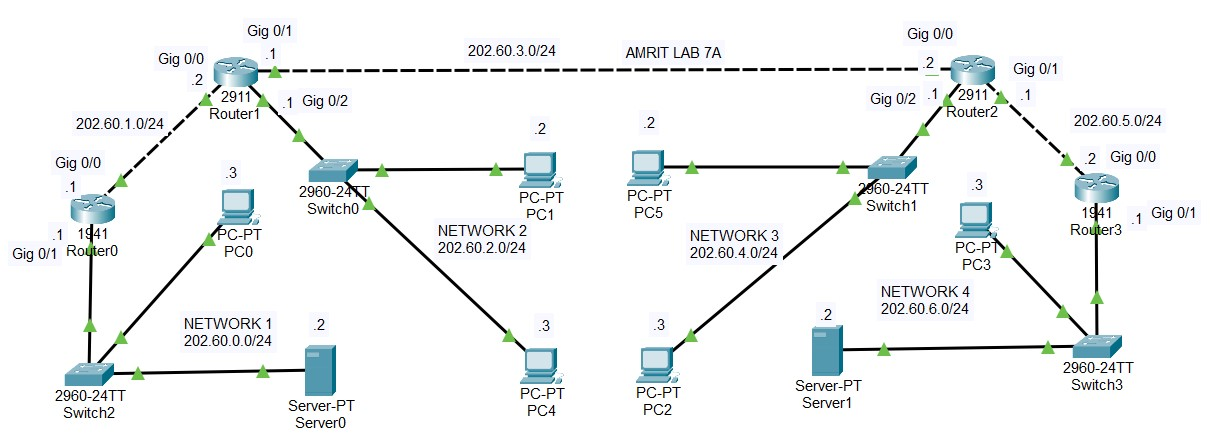
\includegraphics[scale=0.7,cframe=blue 0.5pt 3pt]{./FIG/Lab7A.jpg}
    \caption{Network topology Lab 7A}
\end{figure}

\begin{enumerate}
    %%%%%%%%%%%%%%%%%%%%%%%%%%%%%%AAAAAAAAAAAAAAAAAAAAAAAAAAAAAAA11111111111111111111111
    \item\textbf{Configure the hostname, console password and enable password in each Router.}

          \addtocontents{lol}{\protect\subsubsection*{A.1 : Routers Configuration}}

          \CMD{./CODES/A_config0.txt}{Config Hostname, Console ,enable,vty password for Router 0}

          % \usepackage{colortbl}

          \begin{table}[H]
              \centering
              \begin{tabular} {| m{6em}| m{6em}| m{9em} | m{8em}| m{7em} |}
                  \hline
                  {\cellcolor[rgb]{0.278,0.671,0.984}}\textbf{S.N} & \textbf{Hostname} & \textbf{Console Password} & \textbf{Enable Password} & \textbf{vty Password} \\
                  \hline
                  {\cellcolor[rgb]{0.278,0.671,0.984}}Router 0     & AMRIT\_0          & amrit                     & 403                      & phuyal                \\
                  \hline
                  {\cellcolor[rgb]{0.278,0.671,0.984}}Router 1     & AMRIT\_1          & amrit                     & 403                      & phuyal                \\
                  \hline
                  {\cellcolor[rgb]{0.278,0.671,0.984}}Router 2     & AMRIT\_2          & amrit                     & 403                      & phuyal                \\
                  \hline
                  {\cellcolor[rgb]{0.278,0.671,0.984}}Router 3     & AMRIT\_3          & amrit                     & 403                      & phuyal                \\
                  \hline
              \end{tabular}
              \caption{Table for hostname, console password , enable password,vty password}
          \end{table}


          %%%%%%%%%%%%%%%%%%%%%%%%%%%%%%AAAAAAAAAAAAAAAAAAAAAAAAAAAAAAA222222222222222222222222222
    \item\textbf{ Configure each interfaces of Router with given IP address and appropriate interface  description.}

          \addtocontents{lol}{\protect\subsubsection*{A.2 : Assign IP to Interfaces}}
          \CMD{./CODES/A_IP0.txt}{Configuring each interface of Router0}
          \CMD{./CODES/A_IP3.txt}{Configuring each interface of Router3}
          % \usepackage{colortbl}
          % \usepackage{multirow}
          % \usepackage{hhline}



          \begin{table}[H]
              \centering
              \
              \begin{tabular}{|l|l|l|l|}
                  \hline
                  \rowcolor[rgb]{0.443,0.831,1} \textbf{Router no.} & {\cellcolor[rgb]{0.325,1,0.784}}\textbf{GigabitEthernet} & \textbf{Assigned Ip} & \textbf{Description}    \\
                  \hline
                  \multirow{2}{*}{\textbf{Router 0~ }}              & {\cellcolor[rgb]{0.325,1,0.784}}0/0                      & 202.60.1.1           & Connected to Router 1~~ \\
                  \hhline{|~---|}
                                                                    & {\cellcolor[rgb]{0.325,1,0.784}}0/1                      & 202.60.0.1           & Connected to Network 1  \\
                  \hline
                  \multirow{3}{*}{\textbf{Router 1~~ }}             & {\cellcolor[rgb]{0.325,1,0.784}}0/0                      & 202.60.1.2           & Connected to Router 0   \\
                  \hhline{|~---|}
                                                                    & {\cellcolor[rgb]{0.325,1,0.784}}0/1                      & 202.60.3.1           & Connected to Router 2   \\
                  \hhline{|~---|}
                                                                    & {\cellcolor[rgb]{0.325,1,0.784}}0/2                      & 202.60.2.1           & Connected to Network 2  \\
                  \hline
                  \multirow{3}{*}{\textbf{~Router 2~~ }}            & {\cellcolor[rgb]{0.325,1,0.784}}0/0                      & 202.60.3.2           & Connected to Router 1   \\
                  \hhline{|~---|}
                                                                    & {\cellcolor[rgb]{0.325,1,0.784}}0/1                      & 202.60.5.1           & Connected to Router 3   \\
                  \hhline{|~---|}
                                                                    & {\cellcolor[rgb]{0.325,1,0.784}}0/2                      & 202.60.4.1           & Connected to Network 3  \\
                  \hline
                  \multirow{2}{*}{\textbf{Router 3 }}               & {\cellcolor[rgb]{0.325,1,0.784}}0/0                      & 202.60.5.2           & Connected to Router 2   \\
                  \hhline{|~---|}
                                                                    & {\cellcolor[rgb]{0.325,1,0.784}}0/1                      & 202.60.6.1           & Connected to Network 4  \\
                  \hline
              \end{tabular}
              \caption{Assigned IPs and description for all interfaces}
          \end{table}


          %%%%%%%%%%%%%%%%%%%%%%%%%%%%%%AAAAAAAAAAAAAAAAAAAAAAAAAAAAA3333333333333333333333333333333
    \item\textbf{ Configure the IP address and default gateway on each computer as specified in figure above. }

          % \usepackage{multirow}
          % \usepackage{colortbl}
          % \usepackage{hhline}


          \begin{table}[H]
              \centering

              \arrayrulecolor{black}
              \begin{tabular}{| m{6em}| m{8em}| m{9em} | m{8em} |}
                  \hline
                  \rowcolor[rgb]{0.235,1,0.808} \textbf{Network no.~}         & \textbf{Default gateway}    & \textbf{~Device name} & \textbf{Assigned IP} \\
                  \hline
                  {\cellcolor[rgb]{0.259,0.753,1}}                            & \multirow{2}{*}{202.60.0.1} & Server 0              & 202.60.0.2           \\
                  \hhline{|>{\arrayrulecolor[rgb]{0.259,0.753,1}}-~>{\arrayrulecolor{black}}--|}
                  \multirow{-2}{*}{{\cellcolor[rgb]{0.259,0.753,1}}Network 1} &                             & PC0                   & 202.60.0.3           \\
                  \hline
                  {\cellcolor[rgb]{0.259,0.753,1}}                            & \multirow{2}{*}{202.60.2.1} & PC1                   & 202.60.2.2           \\
                  \hhline{|>{\arrayrulecolor[rgb]{0.259,0.753,1}}-~>{\arrayrulecolor{black}}--|}
                  \multirow{-2}{*}{{\cellcolor[rgb]{0.259,0.753,1}}Network 2} &                             & PC4                   & 202.60.2.3           \\
                  \hline
                  {\cellcolor[rgb]{0.259,0.753,1}}                            & \multirow{2}{*}{202.60.4.1} & PC5                   & 202.60.4.2           \\
                  \hhline{|>{\arrayrulecolor[rgb]{0.259,0.753,1}}-~>{\arrayrulecolor{black}}--|}
                  \multirow{-2}{*}{{\cellcolor[rgb]{0.259,0.753,1}}Network 3} &                             & PC2                   & 202.60.4.3           \\
                  \hline
                  {\cellcolor[rgb]{0.259,0.753,1}}                            & \multirow{2}{*}{202.60.6.1} & Server 1              & 202.60.6.2           \\
                  \hhline{|>{\arrayrulecolor[rgb]{0.259,0.753,1}}-~>{\arrayrulecolor{black}}--|}
                  \multirow{-2}{*}{{\cellcolor[rgb]{0.259,0.753,1}}Network 4} &                             & PC3                   & 202.60.6.3           \\
                  \hline
              \end{tabular}
              \caption{Table for Name, assigned ip, Default gateway}
          \end{table}

          %%%%%%%%%%%%%%%%%%%%%%%%%%%%%%AAAAAAAAAAAAAAAAAAAAAAAAAAAAAAA44444444444444444444444444444
    \item\textbf{ Enable telnet on each Router. }

          Already enabled in Activity A.1

          %%%%%%%%%%%%%%%%%%%%%%%%%%%%%%AAAAAAAAAAAAAAAAAAAAAAAAAAAAAAA55555555555555555555555555555
    \item\textbf{ Observe the output of the command \textit{show ip route} in each Router and note it down.}
          \addtocontents{lol}{\protect\subsubsection*{A.5 : Routing table of Routers}}
          \CMD{./CODES/A_Showip0.txt}{\textit{show ip route} Router 0}
          \CMD{./CODES/A_Showip1.txt}{\textit{show ip route} Router 1}
          \CMD{./CODES/A_Showip2.txt}{\textit{show ip route} Router 2}
          \CMD{./CODES/A_Showip3.txt}{\textit{show ip route} Router 3}

          %%%%%%%%%%%%%%%%%%%%%%%%%%%%%%AAAAAAAAAAAAAAAAAAAAAAAAAAAAAAA666666666666666666666666666
    \item\textbf{ Observe the output while using ping command from PC0 to PC0, PC1, PC2, PC3, Server0,
              Server1, Router0, Router1, Router2 and Router3.
          }
          \addtocontents{lol}{\protect\subsubsection*{A.6 : Ping from PC0}}
          \CMD{./CODES/AP0-r01.txt}{Ping from PC0 to Router 0 : 0/1}

          \CMD{./CODES/AP0-r22.txt}{Ping from PC0 to Router 2 : 0/2}

          \CMD{./CODES/AP0-3.txt}{Ping from PC0 to PC3}

          % \usepackage{colortbl}
          % \usepackage{multirow}
          % \usepackage{hhline}


          \begin{table}[H]
              \centering

              \arrayrulecolor{black}
              \begin{tabular}{| m{9em}| m{12em}| m{9em} |}
                  \hline
                  {\cellcolor[rgb]{0.333,0.686,1}}\textbf{Sending Host}           & \textbf{Destination} & \textbf{Ping status}                                                   \\
                  \hline
                  {\cellcolor[rgb]{0.333,0.686,1}}                                & PC0                  & {\cellcolor[rgb]{0.376,1,0.882}}                                       \\
                  \hhline{|>{\arrayrulecolor[rgb]{0.333,0.686,1}}->{\arrayrulecolor{black}}->{\arrayrulecolor[rgb]{0.376,1,0.882}}->{\arrayrulecolor{black}}|}
                  {\cellcolor[rgb]{0.333,0.686,1}}                                & Server 0             & {\cellcolor[rgb]{0.376,1,0.882}}                                       \\
                  \hhline{|>{\arrayrulecolor[rgb]{0.333,0.686,1}}->{\arrayrulecolor{black}}->{\arrayrulecolor[rgb]{0.376,1,0.882}}->{\arrayrulecolor{black}}|}
                  {\cellcolor[rgb]{0.333,0.686,1}}                                & Router 0 : 0/1       & {\cellcolor[rgb]{0.376,1,0.882}}                                       \\
                  \hhline{|>{\arrayrulecolor[rgb]{0.333,0.686,1}}->{\arrayrulecolor{black}}->{\arrayrulecolor[rgb]{0.376,1,0.882}}->{\arrayrulecolor{black}}|}
                  {\cellcolor[rgb]{0.333,0.686,1}}                                & Router 0 : 0/0       & \multirow{-4}{*}{{\cellcolor[rgb]{0.376,1,0.882}}\textbf{ Successful}} \\
                  \hhline{|>{\arrayrulecolor[rgb]{0.333,0.686,1}}->{\arrayrulecolor{black}}--|}
                  {\cellcolor[rgb]{0.333,0.686,1}}                                & Router 1 : 0/0       & {\cellcolor[rgb]{1,0.173,0.09}}                                        \\
                  \hhline{|>{\arrayrulecolor[rgb]{0.333,0.686,1}}->{\arrayrulecolor{black}}->{\arrayrulecolor[rgb]{1,0.173,0.09}}->{\arrayrulecolor{black}}|}
                  {\cellcolor[rgb]{0.333,0.686,1}}                                & Router 1 : 0/1       & {\cellcolor[rgb]{1,0.173,0.09}}                                        \\
                  \hhline{|>{\arrayrulecolor[rgb]{0.333,0.686,1}}->{\arrayrulecolor{black}}->{\arrayrulecolor[rgb]{1,0.173,0.09}}->{\arrayrulecolor{black}}|}
                  {\cellcolor[rgb]{0.333,0.686,1}}                                & Router 1 : 0/2       & {\cellcolor[rgb]{1,0.173,0.09}}                                        \\
                  \hhline{|>{\arrayrulecolor[rgb]{0.333,0.686,1}}->{\arrayrulecolor{black}}->{\arrayrulecolor[rgb]{1,0.173,0.09}}->{\arrayrulecolor{black}}|}
                  {\cellcolor[rgb]{0.333,0.686,1}}                                & PC1                  & {\cellcolor[rgb]{1,0.173,0.09}}                                        \\
                  \hhline{|>{\arrayrulecolor[rgb]{0.333,0.686,1}}->{\arrayrulecolor{black}}->{\arrayrulecolor[rgb]{1,0.173,0.09}}->{\arrayrulecolor{black}}|}
                  {\cellcolor[rgb]{0.333,0.686,1}}                                & Router 2 : 0/0       & {\cellcolor[rgb]{1,0.173,0.09}}                                        \\
                  \hhline{|>{\arrayrulecolor[rgb]{0.333,0.686,1}}->{\arrayrulecolor{black}}->{\arrayrulecolor[rgb]{1,0.173,0.09}}->{\arrayrulecolor{black}}|}
                  {\cellcolor[rgb]{0.333,0.686,1}}                                & Router 2 : 0/2       & {\cellcolor[rgb]{1,0.173,0.09}}                                        \\
                  \hhline{|>{\arrayrulecolor[rgb]{0.333,0.686,1}}->{\arrayrulecolor{black}}->{\arrayrulecolor[rgb]{1,0.173,0.09}}->{\arrayrulecolor{black}}|}
                  {\cellcolor[rgb]{0.333,0.686,1}}                                & PC2                  & {\cellcolor[rgb]{1,0.173,0.09}}                                        \\
                  \hhline{|>{\arrayrulecolor[rgb]{0.333,0.686,1}}->{\arrayrulecolor{black}}->{\arrayrulecolor[rgb]{1,0.173,0.09}}->{\arrayrulecolor{black}}|}
                  {\cellcolor[rgb]{0.333,0.686,1}}                                & Router 2 : 0/1       & {\cellcolor[rgb]{1,0.173,0.09}}                                        \\
                  \hhline{|>{\arrayrulecolor[rgb]{0.333,0.686,1}}->{\arrayrulecolor{black}}->{\arrayrulecolor[rgb]{1,0.173,0.09}}->{\arrayrulecolor{black}}|}
                  {\cellcolor[rgb]{0.333,0.686,1}}                                & Router 3 : 0/0       & {\cellcolor[rgb]{1,0.173,0.09}}                                        \\
                  \hhline{|>{\arrayrulecolor[rgb]{0.333,0.686,1}}->{\arrayrulecolor{black}}->{\arrayrulecolor[rgb]{1,0.173,0.09}}->{\arrayrulecolor{black}}|}
                  {\cellcolor[rgb]{0.333,0.686,1}}                                & Router 3 : 0/1       & {\cellcolor[rgb]{1,0.173,0.09}}                                        \\
                  \hhline{|>{\arrayrulecolor[rgb]{0.333,0.686,1}}->{\arrayrulecolor{black}}->{\arrayrulecolor[rgb]{1,0.173,0.09}}->{\arrayrulecolor{black}}|}
                  {\cellcolor[rgb]{0.333,0.686,1}}                                & PC3                  & {\cellcolor[rgb]{1,0.173,0.09}}                                        \\
                  \hhline{|>{\arrayrulecolor[rgb]{0.333,0.686,1}}->{\arrayrulecolor{black}}->{\arrayrulecolor[rgb]{1,0.173,0.09}}->{\arrayrulecolor{black}}|}
                  \multirow{-16}{*}{{\cellcolor[rgb]{0.333,0.686,1}}\textbf{PC0}} & Server 1             & \multirow{-12}{*}{{\cellcolor[rgb]{1,0.173,0.09}} \textbf{Failed} }    \\
                  \hline
              \end{tabular}
              \caption{Ping from PC0 to all Routers,PCs and Servers }
          \end{table}


          %%%%%%%%%%%%%%%%%%%%%%%%%%%%%%AAAAAAAAAAAAAAAAAAAAAAAAAAAAAAA777777777777777777777777777777777
    \item\textbf{ Similarly, observe the output while using ping command from PC1 to all other computers,
              servers and routers.
          }

          \addtocontents{lol}{\protect\subsubsection*{A.7 : Ping from PC1}}
          \CMD{./CODES/AP1-r01.txt}{Ping from PC1 to Router 0 : 0/1}

          \CMD{./CODES/AP1-r22.txt}{Ping from PC1 to Router 2 : 0/2}

          \CMD{./CODES/AP1-3.txt}{Ping from PC1 to PC3}


          % \usepackage{colortbl}
          % \usepackage{multirow}
          % \usepackage{hhline}


          \begin{table}[H]
              \centering
              \arrayrulecolor{black}
              \begin{tabular}{| m{9em}| m{12em}| m{9em} |}
                  \hline
                  {\cellcolor[rgb]{0.333,0.686,1}}\textbf{Sending Host}           & \textbf{Destination} & \multicolumn{1}{l|}{\textbf{Ping status}}                                             \\
                  \hline
                  {\cellcolor[rgb]{0.333,0.686,1}}                                & PC0                  & \multicolumn{1}{l|}{{\cellcolor[rgb]{1,0.173,0.09}}}                                  \\
                  \hhline{|>{\arrayrulecolor[rgb]{0.333,0.686,1}}->{\arrayrulecolor{black}}->{\arrayrulecolor[rgb]{1,0.173,0.09}}->{\arrayrulecolor{black}}|}
                  {\cellcolor[rgb]{0.333,0.686,1}}                                & Server 0             & \multicolumn{1}{l|}{{\cellcolor[rgb]{1,0.173,0.09}}}                                  \\
                  \hhline{|>{\arrayrulecolor[rgb]{0.333,0.686,1}}->{\arrayrulecolor{black}}->{\arrayrulecolor[rgb]{1,0.173,0.09}}->{\arrayrulecolor{black}}|}
                  {\cellcolor[rgb]{0.333,0.686,1}}                                & Router 0 : 0/1       & \multicolumn{1}{l|}{{\cellcolor[rgb]{1,0.173,0.09}}}                                  \\
                  \hhline{|>{\arrayrulecolor[rgb]{0.333,0.686,1}}->{\arrayrulecolor{black}}->{\arrayrulecolor[rgb]{1,0.173,0.09}}->{\arrayrulecolor{black}}|}
                  {\cellcolor[rgb]{0.333,0.686,1}}                                & Router 0 : 0/0       & \multicolumn{1}{l|}{\multirow{-4}{*}{{\cellcolor[rgb]{1,0.173,0.09}}\textbf{Failed}}} \\
                  \hhline{|>{\arrayrulecolor[rgb]{0.333,0.686,1}}->{\arrayrulecolor{black}}--}
                  {\cellcolor[rgb]{0.333,0.686,1}}                                & Router 1 : 0/0       & {\cellcolor[rgb]{0.376,1,0.882}}                                                      \\
                  \hhline{|>{\arrayrulecolor[rgb]{0.333,0.686,1}}->{\arrayrulecolor{black}}->{\arrayrulecolor[rgb]{0.376,1,0.882}}-}
                  {\cellcolor[rgb]{0.333,0.686,1}}                                & Router 1 : 0/1       & {\cellcolor[rgb]{0.376,1,0.882}}                                                      \\
                  \hhline{>{\arrayrulecolor{black}}|>{\arrayrulecolor[rgb]{0.333,0.686,1}}->{\arrayrulecolor{black}}->{\arrayrulecolor[rgb]{0.376,1,0.882}}-}
                  {\cellcolor[rgb]{0.333,0.686,1}}                                & Router 1 : 0/2       & {\cellcolor[rgb]{0.376,1,0.882}}                                                      \\
                  \hhline{>{\arrayrulecolor{black}}|>{\arrayrulecolor[rgb]{0.333,0.686,1}}->{\arrayrulecolor{black}}->{\arrayrulecolor[rgb]{0.376,1,0.882}}-}
                  {\cellcolor[rgb]{0.333,0.686,1}}                                & PC1                  & \multirow{-4}{*}{{\cellcolor[rgb]{0.376,1,0.882}}\textbf{Successful}}                 \\
                  \hhline{>{\arrayrulecolor{black}}|>{\arrayrulecolor[rgb]{0.333,0.686,1}}->{\arrayrulecolor{black}}->{\arrayrulecolor[rgb]{1,0.173,0.09}}-}
                  {\cellcolor[rgb]{0.333,0.686,1}}                                & Router 2 : 0/0       & {\cellcolor[rgb]{1,0.173,0.09}}                                                       \\
                  \hhline{>{\arrayrulecolor{black}}|>{\arrayrulecolor[rgb]{0.333,0.686,1}}->{\arrayrulecolor{black}}->{\arrayrulecolor[rgb]{1,0.173,0.09}}-}
                  {\cellcolor[rgb]{0.333,0.686,1}}                                & Router 2 : 0/2       & {\cellcolor[rgb]{1,0.173,0.09}}                                                       \\
                  \hhline{>{\arrayrulecolor{black}}|>{\arrayrulecolor[rgb]{0.333,0.686,1}}->{\arrayrulecolor{black}}->{\arrayrulecolor[rgb]{1,0.173,0.09}}-}
                  {\cellcolor[rgb]{0.333,0.686,1}}                                & PC2                  & {\cellcolor[rgb]{1,0.173,0.09}}                                                       \\
                  \hhline{>{\arrayrulecolor{black}}|>{\arrayrulecolor[rgb]{0.333,0.686,1}}->{\arrayrulecolor{black}}->{\arrayrulecolor[rgb]{1,0.173,0.09}}-}
                  {\cellcolor[rgb]{0.333,0.686,1}}                                & Router 2 : 0/1       & {\cellcolor[rgb]{1,0.173,0.09}}                                                       \\
                  \hhline{>{\arrayrulecolor{black}}|>{\arrayrulecolor[rgb]{0.333,0.686,1}}->{\arrayrulecolor{black}}->{\arrayrulecolor[rgb]{1,0.173,0.09}}-}
                  {\cellcolor[rgb]{0.333,0.686,1}}                                & Router 3 : 0/0       & {\cellcolor[rgb]{1,0.173,0.09}}                                                       \\
                  \hhline{>{\arrayrulecolor{black}}|>{\arrayrulecolor[rgb]{0.333,0.686,1}}->{\arrayrulecolor{black}}->{\arrayrulecolor[rgb]{1,0.173,0.09}}-}
                  {\cellcolor[rgb]{0.333,0.686,1}}                                & Router 3 : 0/1       & {\cellcolor[rgb]{1,0.173,0.09}}                                                       \\
                  \hhline{>{\arrayrulecolor{black}}|>{\arrayrulecolor[rgb]{0.333,0.686,1}}->{\arrayrulecolor{black}}->{\arrayrulecolor[rgb]{1,0.173,0.09}}-}
                  {\cellcolor[rgb]{0.333,0.686,1}}                                & PC3                  & {\cellcolor[rgb]{1,0.173,0.09}}                                                       \\
                  \hhline{>{\arrayrulecolor{black}}|>{\arrayrulecolor[rgb]{0.333,0.686,1}}->{\arrayrulecolor{black}}->{\arrayrulecolor[rgb]{1,0.173,0.09}}-}
                  \multirow{-16}{*}{{\cellcolor[rgb]{0.333,0.686,1}}\textbf{PC1}} & Server 1             & \multirow{-8}{*}{{\cellcolor[rgb]{1,0.173,0.09}}\textbf{ Failed }}                    \\
                  \hhline{>{\arrayrulecolor{black}}|-->{\arrayrulecolor[rgb]{1,0.173,0.09}}-}
              \end{tabular}
              \arrayrulecolor{black}
              \caption{Ping from PC1 to all Routers,PCs and Servers }
          \end{table}




          %%%%%%%%%%%%%%%%%%%%%%%%%%%%%%AAAAAAAAAAAAAAAAAAAAAAAAAAAAAAA888888888888888888888888888
    \item\textbf{ Repeat the process from all other computers and routers.}
          \addtocontents{lol}{\protect\subsubsection*{A.8 : Ping from other PCs and Router}}
          \begin{enumerate}
              \item \textbf{Ping from PC2}

                    \addtocontents{lol}{\protect\subsubsection*{\quad \quad \small  A.8.a : Ping from PC2}}

                    \CMD{./CODES/AP2-r01.txt}{Ping from PC2 to Router 0 : 0/1}

                    \CMD{./CODES/AP2-1.txt}{Ping from PC2 to PC1}

                    \CMD{./CODES/AP2-3.txt}{Ping from PC2 to PC3}

                    % \usepackage{colortbl}
                    % \usepackage{multirow}
                    % \usepackage{hhline}


                    \begin{table}[H]
                        \centering
                        \arrayrulecolor{black}
                        \begin{tabular}{| m{9em}| m{12em}| m{9em} |}
                            \hline
                            {\cellcolor[rgb]{0.333,0.686,1}}\textbf{Sending Host}           & \textbf{Destination} & \textbf{Ping status}                                                                      \\
                            \hline
                            {\cellcolor[rgb]{0.333,0.686,1}}                                & PC0                  & {\cellcolor[rgb]{1,0.173,0.09}}                                                           \\
                            \hhline{|>{\arrayrulecolor[rgb]{0.333,0.686,1}}->{\arrayrulecolor{black}}->{\arrayrulecolor[rgb]{1,0.173,0.09}}->{\arrayrulecolor{black}}|}
                            {\cellcolor[rgb]{0.333,0.686,1}}                                & Server 0             & {\cellcolor[rgb]{1,0.173,0.09}}                                                           \\
                            \hhline{|>{\arrayrulecolor[rgb]{0.333,0.686,1}}->{\arrayrulecolor{black}}->{\arrayrulecolor[rgb]{1,0.173,0.09}}->{\arrayrulecolor{black}}|}
                            {\cellcolor[rgb]{0.333,0.686,1}}                                & Router 0 : 0/1       & {\cellcolor[rgb]{1,0.173,0.09}}                                                           \\
                            \hhline{|>{\arrayrulecolor[rgb]{0.333,0.686,1}}->{\arrayrulecolor{black}}->{\arrayrulecolor[rgb]{1,0.173,0.09}}->{\arrayrulecolor{black}}|}
                            {\cellcolor[rgb]{0.333,0.686,1}}                                & Router 0 : 0/0       & {\cellcolor[rgb]{1,0.173,0.09}}                                                           \\
                            \hhline{|>{\arrayrulecolor[rgb]{0.333,0.686,1}}->{\arrayrulecolor{black}}->{\arrayrulecolor[rgb]{1,0.173,0.09}}->{\arrayrulecolor{black}}|}
                            {\cellcolor[rgb]{0.333,0.686,1}}                                & Router 1 : 0/0       & {\cellcolor[rgb]{1,0.173,0.09}}                                                           \\
                            \hhline{|>{\arrayrulecolor[rgb]{0.333,0.686,1}}->{\arrayrulecolor{black}}->{\arrayrulecolor[rgb]{1,0.173,0.09}}->{\arrayrulecolor{black}}|}
                            {\cellcolor[rgb]{0.333,0.686,1}}                                & Router 1 : 0/1       & {\cellcolor[rgb]{1,0.173,0.09}}                                                           \\
                            \hhline{|>{\arrayrulecolor[rgb]{0.333,0.686,1}}->{\arrayrulecolor{black}}->{\arrayrulecolor[rgb]{1,0.173,0.09}}->{\arrayrulecolor{black}}|}
                            {\cellcolor[rgb]{0.333,0.686,1}}                                & Router 1 : 0/2       & {\cellcolor[rgb]{1,0.173,0.09}}                                                           \\
                            \hhline{|>{\arrayrulecolor[rgb]{0.333,0.686,1}}->{\arrayrulecolor{black}}->{\arrayrulecolor[rgb]{1,0.173,0.09}}->{\arrayrulecolor{black}}|}
                            {\cellcolor[rgb]{0.333,0.686,1}}                                & PC1                  & \multirow{-8}{*}{{\cellcolor[rgb]{1,0.173,0.09}}\textbf{Failed} }                         \\
                            \hhline{|>{\arrayrulecolor[rgb]{0.333,0.686,1}}->{\arrayrulecolor{black}}--}
                            {\cellcolor[rgb]{0.333,0.686,1}}                                & Router 2 : 0/0       & \multicolumn{1}{l}{{\cellcolor[rgb]{0.376,1,0.882}}}                                      \\
                            \hhline{|>{\arrayrulecolor[rgb]{0.333,0.686,1}}->{\arrayrulecolor{black}}->{\arrayrulecolor[rgb]{0.376,1,0.882}}-}
                            {\cellcolor[rgb]{0.333,0.686,1}}                                & Router 2 : 0/2       & \multicolumn{1}{l}{{\cellcolor[rgb]{0.376,1,0.882}}}                                      \\
                            \hhline{>{\arrayrulecolor{black}}|>{\arrayrulecolor[rgb]{0.333,0.686,1}}->{\arrayrulecolor{black}}->{\arrayrulecolor[rgb]{0.376,1,0.882}}-}
                            {\cellcolor[rgb]{0.333,0.686,1}}                                & PC2                  & \multicolumn{1}{l}{{\cellcolor[rgb]{0.376,1,0.882}}}                                      \\
                            \hhline{>{\arrayrulecolor{black}}|>{\arrayrulecolor[rgb]{0.333,0.686,1}}->{\arrayrulecolor{black}}->{\arrayrulecolor[rgb]{0.376,1,0.882}}-}
                            {\cellcolor[rgb]{0.333,0.686,1}}                                & Router 2 : 0/1       & \multicolumn{1}{l}{\multirow{-4}{*}{{\cellcolor[rgb]{0.376,1,0.882}}\textbf{Successful}}} \\
                            \hhline{>{\arrayrulecolor{black}}|>{\arrayrulecolor[rgb]{0.333,0.686,1}}->{\arrayrulecolor{black}}->{\arrayrulecolor[rgb]{1,0.173,0.09}}-}
                            {\cellcolor[rgb]{0.333,0.686,1}}                                & Router 3 : 0/0       & \multicolumn{1}{l}{{\cellcolor[rgb]{1,0.173,0.09}}}                                       \\
                            \hhline{>{\arrayrulecolor{black}}|>{\arrayrulecolor[rgb]{0.333,0.686,1}}->{\arrayrulecolor{black}}->{\arrayrulecolor[rgb]{1,0.173,0.09}}-}
                            {\cellcolor[rgb]{0.333,0.686,1}}                                & Router 3 : 0/1       & \multicolumn{1}{l}{{\cellcolor[rgb]{1,0.173,0.09}}}                                       \\
                            \hhline{>{\arrayrulecolor{black}}|>{\arrayrulecolor[rgb]{0.333,0.686,1}}->{\arrayrulecolor{black}}->{\arrayrulecolor[rgb]{1,0.173,0.09}}-}
                            {\cellcolor[rgb]{0.333,0.686,1}}                                & PC3                  & \multicolumn{1}{l}{{\cellcolor[rgb]{1,0.173,0.09}}}                                       \\
                            \hhline{>{\arrayrulecolor{black}}|>{\arrayrulecolor[rgb]{0.333,0.686,1}}->{\arrayrulecolor{black}}->{\arrayrulecolor[rgb]{1,0.173,0.09}}-}
                            \multirow{-16}{*}{{\cellcolor[rgb]{0.333,0.686,1}}\textbf{PC2}} & Server 1             & \multicolumn{1}{l}{\multirow{-4}{*}{{\cellcolor[rgb]{1,0.173,0.09}}\textbf{Failed}}}      \\
                            \hhline{>{\arrayrulecolor{black}}|-->{\arrayrulecolor[rgb]{1,0.173,0.09}}-}
                        \end{tabular}
                        \caption{Ping from PC2 to all Routers,PCs and Servers }
                        \arrayrulecolor{black}
                    \end{table}





                    %%%%%%%%%%%%%%%%%%%%%%%%%%%%%%AAAAAAAAAAAAAAAAAAAAAAAAAAAAAAA
              \item \textbf{Ping from PC3}

                    \addtocontents{lol}{\protect\subsubsection*{\quad \quad \small  A.8.b : Ping from PC3}}
                    \CMD{./CODES/AP3-r01.txt}{Ping from PC3 to Router 0 : 0/1}

                    \CMD{./CODES/AP3-1.txt}{Ping from PC3 to PC1}

                    \CMD{./CODES/AP3-2.txt}{Ping from PC3 to PC2}

                    \CMD{./CODES/AP3-s1.txt}{Ping from PC3 to Server 1}

                    % \usepackage{colortbl}
                    % \usepackage{multirow}
                    % \usepackage{hhline}


                    \begin{table}[H]
                        \centering

                        \arrayrulecolor{black}
                        \begin{tabular} {| m{9em}| m{12em}| m{9em} |}
                            \hline
                            {\cellcolor[rgb]{0.333,0.686,1}}\textbf{Sending Host}           & \textbf{Destination} & \textbf{Ping status}                                                     \\
                            \hline
                            {\cellcolor[rgb]{0.333,0.686,1}}                                & PC0                  & {\cellcolor[rgb]{1,0.173,0.09}}                                          \\
                            \hhline{|>{\arrayrulecolor[rgb]{0.333,0.686,1}}->{\arrayrulecolor{black}}->{\arrayrulecolor[rgb]{1,0.173,0.09}}->{\arrayrulecolor{black}}|}
                            {\cellcolor[rgb]{0.333,0.686,1}}                                & Server 0             & {\cellcolor[rgb]{1,0.173,0.09}}                                          \\
                            \hhline{|>{\arrayrulecolor[rgb]{0.333,0.686,1}}->{\arrayrulecolor{black}}->{\arrayrulecolor[rgb]{1,0.173,0.09}}->{\arrayrulecolor{black}}|}
                            {\cellcolor[rgb]{0.333,0.686,1}}                                & Router 0 : 0/1       & {\cellcolor[rgb]{1,0.173,0.09}}                                          \\
                            \hhline{|>{\arrayrulecolor[rgb]{0.333,0.686,1}}->{\arrayrulecolor{black}}->{\arrayrulecolor[rgb]{1,0.173,0.09}}->{\arrayrulecolor{black}}|}
                            {\cellcolor[rgb]{0.333,0.686,1}}                                & Router 0 : 0/0       & {\cellcolor[rgb]{1,0.173,0.09}}                                          \\
                            \hhline{|>{\arrayrulecolor[rgb]{0.333,0.686,1}}->{\arrayrulecolor{black}}->{\arrayrulecolor[rgb]{1,0.173,0.09}}->{\arrayrulecolor{black}}|}
                            {\cellcolor[rgb]{0.333,0.686,1}}                                & Router 1 : 0/0       & {\cellcolor[rgb]{1,0.173,0.09}}                                          \\
                            \hhline{|>{\arrayrulecolor[rgb]{0.333,0.686,1}}->{\arrayrulecolor{black}}->{\arrayrulecolor[rgb]{1,0.173,0.09}}->{\arrayrulecolor{black}}|}
                            {\cellcolor[rgb]{0.333,0.686,1}}                                & Router 1 : 0/1       & {\cellcolor[rgb]{1,0.173,0.09}}                                          \\
                            \hhline{|>{\arrayrulecolor[rgb]{0.333,0.686,1}}->{\arrayrulecolor{black}}->{\arrayrulecolor[rgb]{1,0.173,0.09}}->{\arrayrulecolor{black}}|}
                            {\cellcolor[rgb]{0.333,0.686,1}}                                & Router 1 : 0/2       & {\cellcolor[rgb]{1,0.173,0.09}}                                          \\
                            \hhline{|>{\arrayrulecolor[rgb]{0.333,0.686,1}}->{\arrayrulecolor{black}}->{\arrayrulecolor[rgb]{1,0.173,0.09}}->{\arrayrulecolor{black}}|}
                            {\cellcolor[rgb]{0.333,0.686,1}}                                & PC1                  & {\cellcolor[rgb]{1,0.173,0.09}}                                          \\
                            \hhline{|>{\arrayrulecolor[rgb]{0.333,0.686,1}}->{\arrayrulecolor{black}}->{\arrayrulecolor[rgb]{1,0.173,0.09}}->{\arrayrulecolor{black}}|}
                            {\cellcolor[rgb]{0.333,0.686,1}}                                & Router 2 : 0/0       & {\cellcolor[rgb]{1,0.173,0.09}}                                          \\
                            \hhline{|>{\arrayrulecolor[rgb]{0.333,0.686,1}}->{\arrayrulecolor{black}}->{\arrayrulecolor[rgb]{1,0.173,0.09}}->{\arrayrulecolor{black}}|}
                            {\cellcolor[rgb]{0.333,0.686,1}}                                & Router 2 : 0/2       & {\cellcolor[rgb]{1,0.173,0.09}}                                          \\
                            \hhline{|>{\arrayrulecolor[rgb]{0.333,0.686,1}}->{\arrayrulecolor{black}}->{\arrayrulecolor[rgb]{1,0.173,0.09}}->{\arrayrulecolor{black}}|}
                            {\cellcolor[rgb]{0.333,0.686,1}}                                & PC2                  & {\cellcolor[rgb]{1,0.173,0.09}}                                          \\
                            \hhline{|>{\arrayrulecolor[rgb]{0.333,0.686,1}}->{\arrayrulecolor{black}}->{\arrayrulecolor[rgb]{1,0.173,0.09}}->{\arrayrulecolor{black}}|}
                            {\cellcolor[rgb]{0.333,0.686,1}}                                & Router 2 : 0/1       & \multirow{-12}{*}{{\cellcolor[rgb]{1,0.173,0.09}} \textbf{Failed}}       \\
                            \hhline{|>{\arrayrulecolor[rgb]{0.333,0.686,1}}->{\arrayrulecolor{black}}--}
                            {\cellcolor[rgb]{0.333,0.686,1}}                                & Router 3 : 0/0       & \multicolumn{1}{l}{{\cellcolor[rgb]{0.376,1,0.882}}}                     \\
                            \hhline{|>{\arrayrulecolor[rgb]{0.333,0.686,1}}->{\arrayrulecolor{black}}->{\arrayrulecolor[rgb]{0.376,1,0.882}}-}
                            {\cellcolor[rgb]{0.333,0.686,1}}                                & Router 3 : 0/1       & \multicolumn{1}{l}{{\cellcolor[rgb]{0.376,1,0.882}} \textbf{Successful}} \\
                            \hhline{>{\arrayrulecolor{black}}|>{\arrayrulecolor[rgb]{0.333,0.686,1}}->{\arrayrulecolor{black}}->{\arrayrulecolor[rgb]{0.376,1,0.882}}-}
                            {\cellcolor[rgb]{0.333,0.686,1}}                                & PC3                  & \multicolumn{1}{l}{{\cellcolor[rgb]{0.376,1,0.882}}}                     \\
                            \hhline{>{\arrayrulecolor{black}}|>{\arrayrulecolor[rgb]{0.333,0.686,1}}->{\arrayrulecolor{black}}->{\arrayrulecolor[rgb]{0.376,1,0.882}}-}
                            \multirow{-16}{*}{{\cellcolor[rgb]{0.333,0.686,1}}\textbf{PC3}} & Server 1             & \multicolumn{1}{l}{{\cellcolor[rgb]{0.376,1,0.882}}}                     \\
                            \hhline{>{\arrayrulecolor{black}}|-->{\arrayrulecolor[rgb]{0.376,1,0.882}}-}
                        \end{tabular}
                        \arrayrulecolor{black}
                        \caption{Ping from PC3 to all Routers,PCs and Servers}
                    \end{table}



                    %%%%%%%%%%%%%%%%%%%%%%%%%%%%%%AAAAAAAAAAAAAAAAAAAAAAAAAAAAAAA
              \item \textbf{Ping from Router 0}

                    \addtocontents{lol}{\protect\subsubsection*{\quad \quad \small  A.8.c : Ping from Router 0}}

                    \CMD{./CODES/APr0-0.txt}{Ping from Router 0 to PC0}

                    \CMD{./CODES/APr0-1.txt}{Ping from Router 0 to PC1}

                    \CMD{./CODES/APr0-2.txt}{Ping from Router 0 to PC2}

                    \CMD{./CODES/APr0-s1.txt}{Ping from Router 0 to Server 1}

                    % \usepackage{colortbl}
                    % \usepackage{multirow}
                    % \usepackage{hhline}


                    \begin{table}[H]
                        \centering
                        \arrayrulecolor{black}
                        \begin{tabular}{| m{9em}| m{12em}| m{9em} |}
                            \hline
                            {\cellcolor[rgb]{0.333,0.686,1}}\textbf{Sending Host}                & \textbf{Destination} & \textbf{Ping status}                                                  \\
                            \hline
                            {\cellcolor[rgb]{0.333,0.686,1}}                                     & PC0                  & {\cellcolor[rgb]{0.376,1,0.882}}                                      \\
                            \hhline{|>{\arrayrulecolor[rgb]{0.333,0.686,1}}->{\arrayrulecolor{black}}->{\arrayrulecolor[rgb]{0.376,1,0.882}}->{\arrayrulecolor{black}}|}
                            {\cellcolor[rgb]{0.333,0.686,1}}                                     & Server 0             & {\cellcolor[rgb]{0.376,1,0.882}}                                      \\
                            \hhline{|>{\arrayrulecolor[rgb]{0.333,0.686,1}}->{\arrayrulecolor{black}}->{\arrayrulecolor[rgb]{0.376,1,0.882}}->{\arrayrulecolor{black}}|}
                            {\cellcolor[rgb]{0.333,0.686,1}}                                     & Router 0 : 0/1       & {\cellcolor[rgb]{0.376,1,0.882}}                                      \\
                            \hhline{|>{\arrayrulecolor[rgb]{0.333,0.686,1}}->{\arrayrulecolor{black}}->{\arrayrulecolor[rgb]{0.376,1,0.882}}->{\arrayrulecolor{black}}|}
                            {\cellcolor[rgb]{0.333,0.686,1}}                                     & Router 0 : 0/0       & {\cellcolor[rgb]{0.376,1,0.882}}                                      \\
                            \hhline{|>{\arrayrulecolor[rgb]{0.333,0.686,1}}->{\arrayrulecolor{black}}->{\arrayrulecolor[rgb]{0.376,1,0.882}}->{\arrayrulecolor{black}}|}
                            {\cellcolor[rgb]{0.333,0.686,1}}                                     & Router 1 : 0/0       & \multirow{-5}{*}{{\cellcolor[rgb]{0.376,1,0.882}}\textbf{Successful}} \\
                            \hhline{|>{\arrayrulecolor[rgb]{0.333,0.686,1}}->{\arrayrulecolor{black}}--|}
                            {\cellcolor[rgb]{0.333,0.686,1}}                                     & Router 1 : 0/1       & {\cellcolor[rgb]{1,0.141,0.059}}                                      \\
                            \hhline{|>{\arrayrulecolor[rgb]{0.333,0.686,1}}->{\arrayrulecolor{black}}->{\arrayrulecolor[rgb]{1,0.141,0.059}}->{\arrayrulecolor{black}}|}
                            {\cellcolor[rgb]{0.333,0.686,1}}                                     & Router 1 : 0/2       & {\cellcolor[rgb]{1,0.141,0.059}}                                      \\
                            \hhline{|>{\arrayrulecolor[rgb]{0.333,0.686,1}}->{\arrayrulecolor{black}}->{\arrayrulecolor[rgb]{1,0.141,0.059}}->{\arrayrulecolor{black}}|}
                            {\cellcolor[rgb]{0.333,0.686,1}}                                     & PC1                  & {\cellcolor[rgb]{1,0.141,0.059}}                                      \\
                            \hhline{|>{\arrayrulecolor[rgb]{0.333,0.686,1}}->{\arrayrulecolor{black}}->{\arrayrulecolor[rgb]{1,0.141,0.059}}->{\arrayrulecolor{black}}|}
                            {\cellcolor[rgb]{0.333,0.686,1}}                                     & Router 2 : 0/0       & {\cellcolor[rgb]{1,0.141,0.059}}                                      \\
                            \hhline{|>{\arrayrulecolor[rgb]{0.333,0.686,1}}->{\arrayrulecolor{black}}->{\arrayrulecolor[rgb]{1,0.141,0.059}}->{\arrayrulecolor{black}}|}
                            {\cellcolor[rgb]{0.333,0.686,1}}                                     & Router 2 : 0/2       & {\cellcolor[rgb]{1,0.141,0.059}}                                      \\
                            \hhline{|>{\arrayrulecolor[rgb]{0.333,0.686,1}}->{\arrayrulecolor{black}}->{\arrayrulecolor[rgb]{1,0.141,0.059}}->{\arrayrulecolor{black}}|}
                            {\cellcolor[rgb]{0.333,0.686,1}}                                     & PC2                  & {\cellcolor[rgb]{1,0.141,0.059}}                                      \\
                            \hhline{|>{\arrayrulecolor[rgb]{0.333,0.686,1}}->{\arrayrulecolor{black}}->{\arrayrulecolor[rgb]{1,0.141,0.059}}->{\arrayrulecolor{black}}|}
                            {\cellcolor[rgb]{0.333,0.686,1}}                                     & Router 2 : 0/1       & {\cellcolor[rgb]{1,0.141,0.059}}                                      \\
                            \hhline{|>{\arrayrulecolor[rgb]{0.333,0.686,1}}->{\arrayrulecolor{black}}->{\arrayrulecolor[rgb]{1,0.141,0.059}}->{\arrayrulecolor{black}}|}
                            {\cellcolor[rgb]{0.333,0.686,1}}                                     & Router 3 : 0/0       & {\cellcolor[rgb]{1,0.141,0.059}}                                      \\
                            \hhline{|>{\arrayrulecolor[rgb]{0.333,0.686,1}}->{\arrayrulecolor{black}}->{\arrayrulecolor[rgb]{1,0.141,0.059}}->{\arrayrulecolor{black}}|}
                            {\cellcolor[rgb]{0.333,0.686,1}}                                     & Router 3 : 0/1       & {\cellcolor[rgb]{1,0.141,0.059}}                                      \\
                            \hhline{|>{\arrayrulecolor[rgb]{0.333,0.686,1}}->{\arrayrulecolor{black}}->{\arrayrulecolor[rgb]{1,0.141,0.059}}->{\arrayrulecolor{black}}|}
                            {\cellcolor[rgb]{0.333,0.686,1}}                                     & PC3                  & {\cellcolor[rgb]{1,0.141,0.059}}                                      \\
                            \hhline{|>{\arrayrulecolor[rgb]{0.333,0.686,1}}->{\arrayrulecolor{black}}->{\arrayrulecolor[rgb]{1,0.141,0.059}}->{\arrayrulecolor{black}}|}
                            \multirow{-16}{*}{{\cellcolor[rgb]{0.333,0.686,1}}\textbf{Router 0}} & Server 1             & \multirow{-11}{*}{{\cellcolor[rgb]{1,0.141,0.059}} \textbf{Failed}}   \\
                            \hline
                        \end{tabular}
                        \caption{Ping from Router 0 to all Routers,PCs and Servers }
                    \end{table}


              \item \textbf{Ping from Router 1}

                    \addtocontents{lol}{\protect\subsubsection*{\quad \quad \small  A.8.d : Ping from Router 1}}

                    \CMD{./CODES/APr1-0.txt}{Ping from Router 1 to PC0}

                    \CMD{./CODES/APr1-1.txt}{Ping from Router 1 to PC1}

                    \CMD{./CODES/APr1-r21.txt}{Ping from Router 1 to Router 2: 0/1}

                    \CMD{./CODES/APr1-s1.txt}{Ping from Router 1 to Server 1}

                    % \usepackage{colortbl}
                    % \usepackage{multirow}
                    % \usepackage{hhline}


                    \begin{table}[H]
                        \centering
                        \arrayrulecolor{black}
                        \begin{tabular}{| m{9em}| m{12em}| m{9em} |}
                            \hline
                            {\cellcolor[rgb]{0.333,0.686,1}}\textbf{Sending Host}                & \textbf{Destination} & \multicolumn{1}{l|}{\textbf{Ping status}}                                               \\
                            \hline
                            {\cellcolor[rgb]{0.333,0.686,1}}                                     & PC0                  & \multicolumn{1}{l|}{{\cellcolor[rgb]{1,0.141,0.059}}}                                   \\
                            \hhline{|>{\arrayrulecolor[rgb]{0.333,0.686,1}}->{\arrayrulecolor{black}}->{\arrayrulecolor[rgb]{1,0.141,0.059}}->{\arrayrulecolor{black}}|}
                            {\cellcolor[rgb]{0.333,0.686,1}}                                     & Server 0             & \multicolumn{1}{l|}{{\cellcolor[rgb]{1,0.141,0.059}}}                                   \\
                            \hhline{|>{\arrayrulecolor[rgb]{0.333,0.686,1}}->{\arrayrulecolor{black}}->{\arrayrulecolor[rgb]{1,0.141,0.059}}->{\arrayrulecolor{black}}|}
                            {\cellcolor[rgb]{0.333,0.686,1}}                                     & Router 0 : 0/1       & \multicolumn{1}{l|}{\multirow{-3}{*}{{\cellcolor[rgb]{1,0.141,0.059}}\textbf{Failed} }} \\
                            \hhline{|>{\arrayrulecolor[rgb]{0.333,0.686,1}}->{\arrayrulecolor{black}}--}
                            {\cellcolor[rgb]{0.333,0.686,1}}                                     & Router 0 : 0/0       & {\cellcolor[rgb]{0.376,1,0.882}}                                                        \\
                            \hhline{|>{\arrayrulecolor[rgb]{0.333,0.686,1}}->{\arrayrulecolor{black}}->{\arrayrulecolor[rgb]{0.376,1,0.882}}-}
                            {\cellcolor[rgb]{0.333,0.686,1}}                                     & Router 1 : 0/0       & {\cellcolor[rgb]{0.376,1,0.882}}                                                        \\
                            \hhline{>{\arrayrulecolor{black}}|>{\arrayrulecolor[rgb]{0.333,0.686,1}}->{\arrayrulecolor{black}}->{\arrayrulecolor[rgb]{0.376,1,0.882}}-}
                            {\cellcolor[rgb]{0.333,0.686,1}}                                     & Router 1 : 0/1       & {\cellcolor[rgb]{0.376,1,0.882}}                                                        \\
                            \hhline{>{\arrayrulecolor{black}}|>{\arrayrulecolor[rgb]{0.333,0.686,1}}->{\arrayrulecolor{black}}->{\arrayrulecolor[rgb]{0.376,1,0.882}}-}
                            {\cellcolor[rgb]{0.333,0.686,1}}                                     & Router 1 : 0/2       & {\cellcolor[rgb]{0.376,1,0.882}}                                                        \\
                            \hhline{>{\arrayrulecolor{black}}|>{\arrayrulecolor[rgb]{0.333,0.686,1}}->{\arrayrulecolor{black}}->{\arrayrulecolor[rgb]{0.376,1,0.882}}-}
                            {\cellcolor[rgb]{0.333,0.686,1}}                                     & PC1                  & {\cellcolor[rgb]{0.376,1,0.882}}                                                        \\
                            \hhline{>{\arrayrulecolor{black}}|>{\arrayrulecolor[rgb]{0.333,0.686,1}}->{\arrayrulecolor{black}}->{\arrayrulecolor[rgb]{0.376,1,0.882}}-}
                            {\cellcolor[rgb]{0.333,0.686,1}}                                     & Router 2 : 0/0       & \multirow{-6}{*}{{\cellcolor[rgb]{0.376,1,0.882}}\textbf{Successful}}                   \\
                            \hhline{>{\arrayrulecolor{black}}|>{\arrayrulecolor[rgb]{0.333,0.686,1}}->{\arrayrulecolor{black}}->{\arrayrulecolor[rgb]{1,0.141,0.059}}-}
                            {\cellcolor[rgb]{0.333,0.686,1}}                                     & Router 2 : 0/2       & {\cellcolor[rgb]{1,0.141,0.059}}                                                        \\
                            \hhline{>{\arrayrulecolor{black}}|>{\arrayrulecolor[rgb]{0.333,0.686,1}}->{\arrayrulecolor{black}}->{\arrayrulecolor[rgb]{1,0.141,0.059}}-}
                            {\cellcolor[rgb]{0.333,0.686,1}}                                     & PC2                  & {\cellcolor[rgb]{1,0.141,0.059}}                                                        \\
                            \hhline{>{\arrayrulecolor{black}}|>{\arrayrulecolor[rgb]{0.333,0.686,1}}->{\arrayrulecolor{black}}->{\arrayrulecolor[rgb]{1,0.141,0.059}}-}
                            {\cellcolor[rgb]{0.333,0.686,1}}                                     & Router 2 : 0/1       & {\cellcolor[rgb]{1,0.141,0.059}}                                                        \\
                            \hhline{>{\arrayrulecolor{black}}|>{\arrayrulecolor[rgb]{0.333,0.686,1}}->{\arrayrulecolor{black}}->{\arrayrulecolor[rgb]{1,0.141,0.059}}-}
                            {\cellcolor[rgb]{0.333,0.686,1}}                                     & Router 3 : 0/0       & {\cellcolor[rgb]{1,0.141,0.059}}                                                        \\
                            \hhline{>{\arrayrulecolor{black}}|>{\arrayrulecolor[rgb]{0.333,0.686,1}}->{\arrayrulecolor{black}}->{\arrayrulecolor[rgb]{1,0.141,0.059}}-}
                            {\cellcolor[rgb]{0.333,0.686,1}}                                     & Router 3 : 0/1       & {\cellcolor[rgb]{1,0.141,0.059}}                                                        \\
                            \hhline{>{\arrayrulecolor{black}}|>{\arrayrulecolor[rgb]{0.333,0.686,1}}->{\arrayrulecolor{black}}->{\arrayrulecolor[rgb]{1,0.141,0.059}}-}
                            {\cellcolor[rgb]{0.333,0.686,1}}                                     & PC3                  & {\cellcolor[rgb]{1,0.141,0.059}}                                                        \\
                            \hhline{>{\arrayrulecolor{black}}|>{\arrayrulecolor[rgb]{0.333,0.686,1}}->{\arrayrulecolor{black}}->{\arrayrulecolor[rgb]{1,0.141,0.059}}-}
                            \multirow{-16}{*}{{\cellcolor[rgb]{0.333,0.686,1}}\textbf{Router 1}} & Server 1             & \multirow{-7}{*}{{\cellcolor[rgb]{1,0.141,0.059}}\textbf{Failed}}                       \\
                            \hhline{>{\arrayrulecolor{black}}|-->{\arrayrulecolor[rgb]{1,0.141,0.059}}-}
                        \end{tabular}
                        \caption{Ping from Router 1 to all Routers,PCs and Servers }
                        \arrayrulecolor{black}
                    \end{table}

                    %%%%%%%%%%%%%%%%%%%%%%%%%%%%%%

              \item \textbf{Ping from Router 2}

                    \addtocontents{lol}{\protect\subsubsection*{\quad \quad \small  A.8.e : Ping from Router 2}}
                    \CMD{./CODES/APr2-0.txt}{Ping from Router 2 to PC0}

                    \CMD{./CODES/APr2-r10.txt}{Ping from Router 2 to Router 1 : 0/0}

                    \CMD{./CODES/APr2-2.txt}{Ping from Router 2 to PC2}

                    \CMD{./CODES/APr2-3.txt}{Ping from Router 2 to PC3}


                    % \usepackage{colortbl}
                    % \usepackage{multirow}
                    % \usepackage{hhline}


                    \begin{table}[H]
                        \centering
                        \arrayrulecolor{black}
                        \begin{tabular}{| m{9em}| m{12em}| m{9em} |}
                            \hline
                            {\cellcolor[rgb]{0.333,0.686,1}}\textbf{Sending Host}                & \textbf{Destination} & \multicolumn{1}{l|}{\textbf{Ping status}}                                               \\
                            \hline
                            {\cellcolor[rgb]{0.333,0.686,1}}                                     & PC0                  & \multicolumn{1}{l|}{{\cellcolor[rgb]{1,0.141,0.059}}}                                   \\
                            \hhline{|>{\arrayrulecolor[rgb]{0.333,0.686,1}}->{\arrayrulecolor{black}}->{\arrayrulecolor[rgb]{1,0.141,0.059}}->{\arrayrulecolor{black}}|}
                            {\cellcolor[rgb]{0.333,0.686,1}}                                     & Server 0             & \multicolumn{1}{l|}{{\cellcolor[rgb]{1,0.141,0.059}}}                                   \\
                            \hhline{|>{\arrayrulecolor[rgb]{0.333,0.686,1}}->{\arrayrulecolor{black}}->{\arrayrulecolor[rgb]{1,0.141,0.059}}->{\arrayrulecolor{black}}|}
                            {\cellcolor[rgb]{0.333,0.686,1}}                                     & Router 0 : 0/1       & \multicolumn{1}{l|}{{\cellcolor[rgb]{1,0.141,0.059}}}                                   \\
                            \hhline{|>{\arrayrulecolor[rgb]{0.333,0.686,1}}->{\arrayrulecolor{black}}->{\arrayrulecolor[rgb]{1,0.141,0.059}}->{\arrayrulecolor{black}}|}
                            {\cellcolor[rgb]{0.333,0.686,1}}                                     & Router 0 : 0/0       & \multicolumn{1}{l|}{{\cellcolor[rgb]{1,0.141,0.059}}}                                   \\
                            \hhline{|>{\arrayrulecolor[rgb]{0.333,0.686,1}}->{\arrayrulecolor{black}}->{\arrayrulecolor[rgb]{1,0.141,0.059}}->{\arrayrulecolor{black}}|}
                            {\cellcolor[rgb]{0.333,0.686,1}}                                     & Router 1 : 0/0       & \multicolumn{1}{l|}{\multirow{-5}{*}{{\cellcolor[rgb]{1,0.141,0.059}}\textbf{Failed} }} \\
                            \hhline{|>{\arrayrulecolor[rgb]{0.333,0.686,1}}->{\arrayrulecolor{black}}--}
                            {\cellcolor[rgb]{0.333,0.686,1}}                                     & Router 1 : 0/1       & {\cellcolor[rgb]{0.376,1,0.882}}\textbf{Successful}                                     \\
                            \hhline{|>{\arrayrulecolor[rgb]{0.333,0.686,1}}->{\arrayrulecolor{black}}->{\arrayrulecolor[rgb]{1,0.141,0.059}}-}
                            {\cellcolor[rgb]{0.333,0.686,1}}                                     & Router 1 : 0/2       & {\cellcolor[rgb]{1,0.141,0.059}}                                                        \\
                            \hhline{>{\arrayrulecolor{black}}|>{\arrayrulecolor[rgb]{0.333,0.686,1}}->{\arrayrulecolor{black}}->{\arrayrulecolor[rgb]{1,0.141,0.059}}-}
                            {\cellcolor[rgb]{0.333,0.686,1}}                                     & PC1                  & \multirow{-2}{*}{{\cellcolor[rgb]{1,0.141,0.059}}\textbf{Failed}}                       \\
                            \hhline{>{\arrayrulecolor{black}}|>{\arrayrulecolor[rgb]{0.333,0.686,1}}->{\arrayrulecolor{black}}->{\arrayrulecolor[rgb]{0.376,1,0.882}}-}
                            {\cellcolor[rgb]{0.333,0.686,1}}                                     & Router 2 : 0/0       & {\cellcolor[rgb]{0.376,1,0.882}}                                                        \\
                            \hhline{>{\arrayrulecolor{black}}|>{\arrayrulecolor[rgb]{0.333,0.686,1}}->{\arrayrulecolor{black}}->{\arrayrulecolor[rgb]{0.376,1,0.882}}-}
                            {\cellcolor[rgb]{0.333,0.686,1}}                                     & Router 2 : 0/2       & {\cellcolor[rgb]{0.376,1,0.882}}                                                        \\
                            \hhline{>{\arrayrulecolor{black}}|>{\arrayrulecolor[rgb]{0.333,0.686,1}}->{\arrayrulecolor{black}}->{\arrayrulecolor[rgb]{0.376,1,0.882}}-}
                            {\cellcolor[rgb]{0.333,0.686,1}}                                     & PC2                  & {\cellcolor[rgb]{0.376,1,0.882}}                                                        \\
                            \hhline{>{\arrayrulecolor{black}}|>{\arrayrulecolor[rgb]{0.333,0.686,1}}->{\arrayrulecolor{black}}->{\arrayrulecolor[rgb]{0.376,1,0.882}}-}
                            {\cellcolor[rgb]{0.333,0.686,1}}                                     & Router 2 : 0/1       & {\cellcolor[rgb]{0.376,1,0.882}}                                                        \\
                            \hhline{>{\arrayrulecolor{black}}|>{\arrayrulecolor[rgb]{0.333,0.686,1}}->{\arrayrulecolor{black}}->{\arrayrulecolor[rgb]{0.376,1,0.882}}-}
                            {\cellcolor[rgb]{0.333,0.686,1}}                                     & Router 3 : 0/0       & \multirow{-5}{*}{{\cellcolor[rgb]{0.376,1,0.882}}\textbf{Successful}}                   \\
                            \hhline{>{\arrayrulecolor{black}}|>{\arrayrulecolor[rgb]{0.333,0.686,1}}->{\arrayrulecolor{black}}->{\arrayrulecolor[rgb]{1,0.141,0.059}}-}
                            {\cellcolor[rgb]{0.333,0.686,1}}                                     & Router 3 : 0/1       & {\cellcolor[rgb]{1,0.141,0.059}}                                                        \\
                            \hhline{>{\arrayrulecolor{black}}|>{\arrayrulecolor[rgb]{0.333,0.686,1}}->{\arrayrulecolor{black}}->{\arrayrulecolor[rgb]{1,0.141,0.059}}-}
                            {\cellcolor[rgb]{0.333,0.686,1}}                                     & PC3                  & {\cellcolor[rgb]{1,0.141,0.059}}                                                        \\
                            \hhline{>{\arrayrulecolor{black}}|>{\arrayrulecolor[rgb]{0.333,0.686,1}}->{\arrayrulecolor{black}}->{\arrayrulecolor[rgb]{1,0.141,0.059}}-}
                            \multirow{-16}{*}{{\cellcolor[rgb]{0.333,0.686,1}}\textbf{Router 2}} & Server 1             & \multirow{-3}{*}{{\cellcolor[rgb]{1,0.141,0.059}}\textbf{Failed}}                       \\
                            \hhline{>{\arrayrulecolor{black}}|-->{\arrayrulecolor[rgb]{1,0.141,0.059}}-}
                        \end{tabular}
                        \caption{Ping from Router 2 to all Routers,PCs and Servers }
                        \arrayrulecolor{black}
                    \end{table}


                    %%%%%%%%%%%%%%%%%%%%%%%%%%%%%%

              \item \textbf{Ping from Router 3}

                    \addtocontents{lol}{\protect\subsubsection*{\quad \quad \small  A.8.f : Ping from Router 3}}

                    \CMD{./CODES/APr3-0.txt}{Ping from Router 3 to PC0}

                    \CMD{./CODES/APr3-1.txt}{Ping from Router 3 to PC1}

                    \CMD{./CODES/APr3-2.txt}{Ping from Router 3 to PC2}

                    \CMD{./CODES/APr3-s1.txt}{Ping from Router 3 to Server 1}

                    % \usepackage{colortbl}
                    % \usepackage{multirow}
                    % \usepackage{hhline}



                    \begin{table}[H]
                        \centering
                        \arrayrulecolor{black}
                        \begin{tabular}{| m{9em}| m{12em}| m{9em} |}
                            \hline
                            {\cellcolor[rgb]{0.333,0.686,1}}\textbf{Sending Host}                & \textbf{Destination} & \textbf{Ping status}                                                  \\
                            \hline
                            {\cellcolor[rgb]{0.333,0.686,1}}                                     & PC0                  & {\cellcolor[rgb]{1,0.141,0.059}}                                      \\
                            \hhline{|>{\arrayrulecolor[rgb]{0.333,0.686,1}}->{\arrayrulecolor{black}}->{\arrayrulecolor[rgb]{1,0.141,0.059}}->{\arrayrulecolor{black}}|}
                            {\cellcolor[rgb]{0.333,0.686,1}}                                     & Server 0             & {\cellcolor[rgb]{1,0.141,0.059}}                                      \\
                            \hhline{|>{\arrayrulecolor[rgb]{0.333,0.686,1}}->{\arrayrulecolor{black}}->{\arrayrulecolor[rgb]{1,0.141,0.059}}->{\arrayrulecolor{black}}|}
                            {\cellcolor[rgb]{0.333,0.686,1}}                                     & Router 0 : 0/1       & {\cellcolor[rgb]{1,0.141,0.059}}                                      \\
                            \hhline{|>{\arrayrulecolor[rgb]{0.333,0.686,1}}->{\arrayrulecolor{black}}->{\arrayrulecolor[rgb]{1,0.141,0.059}}->{\arrayrulecolor{black}}|}
                            {\cellcolor[rgb]{0.333,0.686,1}}                                     & Router 0 : 0/0       & {\cellcolor[rgb]{1,0.141,0.059}}                                      \\
                            \hhline{|>{\arrayrulecolor[rgb]{0.333,0.686,1}}->{\arrayrulecolor{black}}->{\arrayrulecolor[rgb]{1,0.141,0.059}}->{\arrayrulecolor{black}}|}
                            {\cellcolor[rgb]{0.333,0.686,1}}                                     & Router 1 : 0/0       & {\cellcolor[rgb]{1,0.141,0.059}}                                      \\
                            \hhline{|>{\arrayrulecolor[rgb]{0.333,0.686,1}}->{\arrayrulecolor{black}}->{\arrayrulecolor[rgb]{1,0.141,0.059}}->{\arrayrulecolor{black}}|}
                            {\cellcolor[rgb]{0.333,0.686,1}}                                     & Router 1 : 0/1       & {\cellcolor[rgb]{1,0.141,0.059}}                                      \\
                            \hhline{|>{\arrayrulecolor[rgb]{0.333,0.686,1}}->{\arrayrulecolor{black}}->{\arrayrulecolor[rgb]{1,0.141,0.059}}->{\arrayrulecolor{black}}|}
                            {\cellcolor[rgb]{0.333,0.686,1}}                                     & Router 1 : 0/2       & {\cellcolor[rgb]{1,0.141,0.059}}                                      \\
                            \hhline{|>{\arrayrulecolor[rgb]{0.333,0.686,1}}->{\arrayrulecolor{black}}->{\arrayrulecolor[rgb]{1,0.141,0.059}}->{\arrayrulecolor{black}}|}
                            {\cellcolor[rgb]{0.333,0.686,1}}                                     & PC1                  & {\cellcolor[rgb]{1,0.141,0.059}}                                      \\
                            \hhline{|>{\arrayrulecolor[rgb]{0.333,0.686,1}}->{\arrayrulecolor{black}}->{\arrayrulecolor[rgb]{1,0.141,0.059}}->{\arrayrulecolor{black}}|}
                            {\cellcolor[rgb]{0.333,0.686,1}}                                     & Router 2 : 0/0       & {\cellcolor[rgb]{1,0.141,0.059}}                                      \\
                            \hhline{|>{\arrayrulecolor[rgb]{0.333,0.686,1}}->{\arrayrulecolor{black}}->{\arrayrulecolor[rgb]{1,0.141,0.059}}->{\arrayrulecolor{black}}|}
                            {\cellcolor[rgb]{0.333,0.686,1}}                                     & Router 2 : 0/2       & {\cellcolor[rgb]{1,0.141,0.059}}                                      \\
                            \hhline{|>{\arrayrulecolor[rgb]{0.333,0.686,1}}->{\arrayrulecolor{black}}->{\arrayrulecolor[rgb]{1,0.141,0.059}}->{\arrayrulecolor{black}}|}
                            {\cellcolor[rgb]{0.333,0.686,1}}                                     & PC2                  & \multirow{-11}{*}{{\cellcolor[rgb]{1,0.141,0.059}}\textbf{Failed} }   \\
                            \hhline{|>{\arrayrulecolor[rgb]{0.333,0.686,1}}->{\arrayrulecolor{black}}--|}
                            {\cellcolor[rgb]{0.333,0.686,1}}                                     & Router 2 : 0/1       & {\cellcolor[rgb]{0.376,1,0.882}}                                      \\
                            \hhline{|>{\arrayrulecolor[rgb]{0.333,0.686,1}}->{\arrayrulecolor{black}}->{\arrayrulecolor[rgb]{0.376,1,0.882}}->{\arrayrulecolor{black}}|}
                            {\cellcolor[rgb]{0.333,0.686,1}}                                     & Router 3 : 0/0       & {\cellcolor[rgb]{0.376,1,0.882}}                                      \\
                            \hhline{|>{\arrayrulecolor[rgb]{0.333,0.686,1}}->{\arrayrulecolor{black}}->{\arrayrulecolor[rgb]{0.376,1,0.882}}->{\arrayrulecolor{black}}|}
                            {\cellcolor[rgb]{0.333,0.686,1}}                                     & Router 3 : 0/1       & {\cellcolor[rgb]{0.376,1,0.882}}                                      \\
                            \hhline{|>{\arrayrulecolor[rgb]{0.333,0.686,1}}->{\arrayrulecolor{black}}->{\arrayrulecolor[rgb]{0.376,1,0.882}}->{\arrayrulecolor{black}}|}
                            {\cellcolor[rgb]{0.333,0.686,1}}                                     & PC3                  & {\cellcolor[rgb]{0.376,1,0.882}}                                      \\
                            \hhline{|>{\arrayrulecolor[rgb]{0.333,0.686,1}}->{\arrayrulecolor{black}}->{\arrayrulecolor[rgb]{0.376,1,0.882}}->{\arrayrulecolor{black}}|}
                            \multirow{-16}{*}{{\cellcolor[rgb]{0.333,0.686,1}}\textbf{Router 3}} & Server 1             & \multirow{-5}{*}{{\cellcolor[rgb]{0.376,1,0.882}}\textbf{Successful}} \\
                            \hline
                        \end{tabular}
                        \caption{Ping from Router 3 to all Routers,PCs and Servers }
                    \end{table}

          \end{enumerate}




          %%%%%%%%%%%%%%%%%%%%%%AAAAAAAAAAAAAAAAAAAAAAAAAA99999999999999999999999999999
    \item\textbf{From PC0 enter into Router0 using telnet and configure RIP.}
          \addtocontents{lol}{\protect\subsubsection*{A.9 : Telnet to Router 0 and configure RIP. }}

          \CMD{./CODES/AT0-0R.txt}{Telnet to Router 0 and configure RIP}



          %%%%%%%%%%%%%%%%%%%%%%%%%%AAAAAAAAAAAAAAAAAAAAAAAAAA10 10 10 10 10 10 1 01 0
    \item\textbf{From there enter into Router1 using telnet and configure RIP.}
          \addtocontents{lol}{\protect\subsubsection*{A.10 : Telnet to Router 1 and configure RIP. }}

          \CMD{./CODES/AT0-1R.txt}{Telnet to Router 1 and configure RIP}


          %%%%%%%%%%%%%%%%%%%%%%%%%%AAAAAAAAAAAAAAAAAAAAAAAAAA11 11 11 11 11 11 11 11 
    \item\textbf{Repeat the process for Router2 and Router3.}
          \addtocontents{lol}{\protect\subsubsection*{A.11 : Telnet to Router 2 and 3 and configure RIP. }}

          From Router 1 we further Telent to Router 2 and Router 3 to configure RIP in them.

          \CMD{./CODES/AT0-2R.txt}{Telnet to Router 2 and configure RIP}

          \CMD{./CODES/AT0-3R.txt}{Telnet to Router 3 and configure RIP}


          %%%%%%%%%%%%%%%%%%%%%%%%%%AAAAAAAAAAAAAAAAAAAAAAAAAA 12 12 12 12 12 12 12 12 12 
    \item\textbf{Repeat the step from 5 to 8 and note down the output by observing it.}
          \addtocontents{lol}{\protect\subsubsection*{A.12 : Repeat the step from 5 to 8 after RIP }}

          \CMD{./CODES/A_Showip0R.txt}{\textit{show ip route} Router 0}
          \CMD{./CODES/A_Showip1R.txt}{\textit{show ip route} Router 1}
          \CMD{./CODES/A_Showip2R.txt}{\textit{show ip route} Router 2}
          \CMD{./CODES/A_Showip3R.txt}{\textit{show ip route} Router 3}

          We can clearly see that there is additional entries in Routing Table in all routers with initial \textbf{R} than available in Activities A.5.  Although we have only configured RIP for connected interface the routing table includes all others routes through communication between the router. In Router 0 we have only entered the neighboring details in Rip but its Routing Table has Routing Path to Network 4.


          \CMD{./CODES/AP0-r22R.txt}{Ping from PC0 to Router 2 : 0/2}

          \begin{table}[H]
              \centering

              \arrayrulecolor{black}
              \begin{tabular}{| m{10em}| m{10em}| m{10em} |}
                  \hline
                  \multicolumn{1}{|l|}{\textbf{Sending Host}}                     & \textbf{Destination} & \multicolumn{1}{l|}{\textbf{Ping Status}}                                  \\
                  \hline
                  {\cellcolor[rgb]{0.141,0.525,1}}                                & PC1                  & {\cellcolor[rgb]{0.42,0.988,0.827}}                                        \\
                  \hhline{|>{\arrayrulecolor[rgb]{0.141,0.525,1}}->{\arrayrulecolor{black}}->{\arrayrulecolor[rgb]{0.42,0.988,0.827}}->{\arrayrulecolor{black}}|}
                  {\cellcolor[rgb]{0.141,0.525,1}}                                & Router 0 : 0/0       & {\cellcolor[rgb]{0.42,0.988,0.827}}                                        \\
                  \hhline{|>{\arrayrulecolor[rgb]{0.141,0.525,1}}->{\arrayrulecolor{black}}->{\arrayrulecolor[rgb]{0.42,0.988,0.827}}->{\arrayrulecolor{black}}|}
                  {\cellcolor[rgb]{0.141,0.525,1}}                                & Router 0 : 0/1       & {\cellcolor[rgb]{0.42,0.988,0.827}}                                        \\
                  \hhline{|>{\arrayrulecolor[rgb]{0.141,0.525,1}}->{\arrayrulecolor{black}}->{\arrayrulecolor[rgb]{0.42,0.988,0.827}}->{\arrayrulecolor{black}}|}
                  {\cellcolor[rgb]{0.141,0.525,1}}                                & Router 0 : 0/2       & {\cellcolor[rgb]{0.42,0.988,0.827}}                                        \\
                  \hhline{|>{\arrayrulecolor[rgb]{0.141,0.525,1}}->{\arrayrulecolor{black}}->{\arrayrulecolor[rgb]{0.42,0.988,0.827}}->{\arrayrulecolor{black}}|}
                  {\cellcolor[rgb]{0.141,0.525,1}}                                & PC3                  & {\cellcolor[rgb]{0.42,0.988,0.827}}                                        \\
                  \hhline{|>{\arrayrulecolor[rgb]{0.141,0.525,1}}->{\arrayrulecolor{black}}->{\arrayrulecolor[rgb]{0.42,0.988,0.827}}->{\arrayrulecolor{black}}|}
                  {\cellcolor[rgb]{0.141,0.525,1}}                                & PC4                  & {\cellcolor[rgb]{0.42,0.988,0.827}}                                        \\
                  \hhline{|>{\arrayrulecolor[rgb]{0.141,0.525,1}}->{\arrayrulecolor{black}}->{\arrayrulecolor[rgb]{0.42,0.988,0.827}}->{\arrayrulecolor{black}}|}
                  {\cellcolor[rgb]{0.141,0.525,1}}                                & Router 1 : 0/0       & {\cellcolor[rgb]{0.42,0.988,0.827}}                                        \\
                  \hhline{|>{\arrayrulecolor[rgb]{0.141,0.525,1}}->{\arrayrulecolor{black}}->{\arrayrulecolor[rgb]{0.42,0.988,0.827}}->{\arrayrulecolor{black}}|}
                  {\cellcolor[rgb]{0.141,0.525,1}}                                & Router 1 : 0/1       & {\cellcolor[rgb]{0.42,0.988,0.827}}                                        \\
                  \hhline{|>{\arrayrulecolor[rgb]{0.141,0.525,1}}->{\arrayrulecolor{black}}->{\arrayrulecolor[rgb]{0.42,0.988,0.827}}->{\arrayrulecolor{black}}|}
                  {\cellcolor[rgb]{0.141,0.525,1}}                                & PC5                  & {\cellcolor[rgb]{0.42,0.988,0.827}}                                        \\
                  \hhline{|>{\arrayrulecolor[rgb]{0.141,0.525,1}}->{\arrayrulecolor{black}}->{\arrayrulecolor[rgb]{0.42,0.988,0.827}}->{\arrayrulecolor{black}}|}
                  \multirow{-10}{*}{{\cellcolor[rgb]{0.141,0.525,1}}\textbf{PC0}} & PC6                  & \multirow{-10}{*}{{\cellcolor[rgb]{0.42,0.988,0.827}} \textbf{Successful}} \\
                  \hline
              \end{tabular}
              \caption{ Ping Status PC0 to all others after RIP}
          \end{table}

          \CMD{./CODES/AP1-3R.txt}{Ping from PC1 to PC3}

          \begin{table}[H]
              \centering

              \arrayrulecolor{black}
              \begin{tabular}{| m{10em}| m{10em}| m{10em} |}
                  \hline
                  \multicolumn{1}{|l|}{\textbf{Sending Host}}                     & \textbf{Destination} & \multicolumn{1}{l|}{\textbf{Ping Status}}                                  \\
                  \hline
                  {\cellcolor[rgb]{0.141,0.525,1}}                                & PC1                  & {\cellcolor[rgb]{0.42,0.988,0.827}}                                        \\
                  \hhline{|>{\arrayrulecolor[rgb]{0.141,0.525,1}}->{\arrayrulecolor{black}}->{\arrayrulecolor[rgb]{0.42,0.988,0.827}}->{\arrayrulecolor{black}}|}
                  {\cellcolor[rgb]{0.141,0.525,1}}                                & Router 0 : 0/0       & {\cellcolor[rgb]{0.42,0.988,0.827}}                                        \\
                  \hhline{|>{\arrayrulecolor[rgb]{0.141,0.525,1}}->{\arrayrulecolor{black}}->{\arrayrulecolor[rgb]{0.42,0.988,0.827}}->{\arrayrulecolor{black}}|}
                  {\cellcolor[rgb]{0.141,0.525,1}}                                & Router 0 : 0/1       & {\cellcolor[rgb]{0.42,0.988,0.827}}                                        \\
                  \hhline{|>{\arrayrulecolor[rgb]{0.141,0.525,1}}->{\arrayrulecolor{black}}->{\arrayrulecolor[rgb]{0.42,0.988,0.827}}->{\arrayrulecolor{black}}|}
                  {\cellcolor[rgb]{0.141,0.525,1}}                                & Router 0 : 0/2       & {\cellcolor[rgb]{0.42,0.988,0.827}}                                        \\
                  \hhline{|>{\arrayrulecolor[rgb]{0.141,0.525,1}}->{\arrayrulecolor{black}}->{\arrayrulecolor[rgb]{0.42,0.988,0.827}}->{\arrayrulecolor{black}}|}
                  {\cellcolor[rgb]{0.141,0.525,1}}                                & PC3                  & {\cellcolor[rgb]{0.42,0.988,0.827}}                                        \\
                  \hhline{|>{\arrayrulecolor[rgb]{0.141,0.525,1}}->{\arrayrulecolor{black}}->{\arrayrulecolor[rgb]{0.42,0.988,0.827}}->{\arrayrulecolor{black}}|}
                  {\cellcolor[rgb]{0.141,0.525,1}}                                & PC4                  & {\cellcolor[rgb]{0.42,0.988,0.827}}                                        \\
                  \hhline{|>{\arrayrulecolor[rgb]{0.141,0.525,1}}->{\arrayrulecolor{black}}->{\arrayrulecolor[rgb]{0.42,0.988,0.827}}->{\arrayrulecolor{black}}|}
                  {\cellcolor[rgb]{0.141,0.525,1}}                                & Router 1 : 0/0       & {\cellcolor[rgb]{0.42,0.988,0.827}}                                        \\
                  \hhline{|>{\arrayrulecolor[rgb]{0.141,0.525,1}}->{\arrayrulecolor{black}}->{\arrayrulecolor[rgb]{0.42,0.988,0.827}}->{\arrayrulecolor{black}}|}
                  {\cellcolor[rgb]{0.141,0.525,1}}                                & Router 1 : 0/1       & {\cellcolor[rgb]{0.42,0.988,0.827}}                                        \\
                  \hhline{|>{\arrayrulecolor[rgb]{0.141,0.525,1}}->{\arrayrulecolor{black}}->{\arrayrulecolor[rgb]{0.42,0.988,0.827}}->{\arrayrulecolor{black}}|}
                  {\cellcolor[rgb]{0.141,0.525,1}}                                & PC5                  & {\cellcolor[rgb]{0.42,0.988,0.827}}                                        \\
                  \hhline{|>{\arrayrulecolor[rgb]{0.141,0.525,1}}->{\arrayrulecolor{black}}->{\arrayrulecolor[rgb]{0.42,0.988,0.827}}->{\arrayrulecolor{black}}|}
                  \multirow{-10}{*}{{\cellcolor[rgb]{0.141,0.525,1}}\textbf{PC1}} & PC6                  & \multirow{-10}{*}{{\cellcolor[rgb]{0.42,0.988,0.827}} \textbf{Successful}} \\
                  \hline
              \end{tabular}
              \caption{ Ping Status PC1 to all others after RIP}
          \end{table}

          \CMD{./CODES/AP2-1R.txt}{Ping from PC2 to PC1}

          \begin{table}[H]
              \centering

              \arrayrulecolor{black}
              \begin{tabular}{| m{10em}| m{10em}| m{10em} |}
                  \hline
                  \multicolumn{1}{|l|}{\textbf{Sending Host}}                     & \textbf{Destination} & \multicolumn{1}{l|}{\textbf{Ping Status}}                                  \\
                  \hline
                  {\cellcolor[rgb]{0.141,0.525,1}}                                & PC1                  & {\cellcolor[rgb]{0.42,0.988,0.827}}                                        \\
                  \hhline{|>{\arrayrulecolor[rgb]{0.141,0.525,1}}->{\arrayrulecolor{black}}->{\arrayrulecolor[rgb]{0.42,0.988,0.827}}->{\arrayrulecolor{black}}|}
                  {\cellcolor[rgb]{0.141,0.525,1}}                                & Router 0 : 0/0       & {\cellcolor[rgb]{0.42,0.988,0.827}}                                        \\
                  \hhline{|>{\arrayrulecolor[rgb]{0.141,0.525,1}}->{\arrayrulecolor{black}}->{\arrayrulecolor[rgb]{0.42,0.988,0.827}}->{\arrayrulecolor{black}}|}
                  {\cellcolor[rgb]{0.141,0.525,1}}                                & Router 0 : 0/1       & {\cellcolor[rgb]{0.42,0.988,0.827}}                                        \\
                  \hhline{|>{\arrayrulecolor[rgb]{0.141,0.525,1}}->{\arrayrulecolor{black}}->{\arrayrulecolor[rgb]{0.42,0.988,0.827}}->{\arrayrulecolor{black}}|}
                  {\cellcolor[rgb]{0.141,0.525,1}}                                & Router 0 : 0/2       & {\cellcolor[rgb]{0.42,0.988,0.827}}                                        \\
                  \hhline{|>{\arrayrulecolor[rgb]{0.141,0.525,1}}->{\arrayrulecolor{black}}->{\arrayrulecolor[rgb]{0.42,0.988,0.827}}->{\arrayrulecolor{black}}|}
                  {\cellcolor[rgb]{0.141,0.525,1}}                                & PC3                  & {\cellcolor[rgb]{0.42,0.988,0.827}}                                        \\
                  \hhline{|>{\arrayrulecolor[rgb]{0.141,0.525,1}}->{\arrayrulecolor{black}}->{\arrayrulecolor[rgb]{0.42,0.988,0.827}}->{\arrayrulecolor{black}}|}
                  {\cellcolor[rgb]{0.141,0.525,1}}                                & PC4                  & {\cellcolor[rgb]{0.42,0.988,0.827}}                                        \\
                  \hhline{|>{\arrayrulecolor[rgb]{0.141,0.525,1}}->{\arrayrulecolor{black}}->{\arrayrulecolor[rgb]{0.42,0.988,0.827}}->{\arrayrulecolor{black}}|}
                  {\cellcolor[rgb]{0.141,0.525,1}}                                & Router 1 : 0/0       & {\cellcolor[rgb]{0.42,0.988,0.827}}                                        \\
                  \hhline{|>{\arrayrulecolor[rgb]{0.141,0.525,1}}->{\arrayrulecolor{black}}->{\arrayrulecolor[rgb]{0.42,0.988,0.827}}->{\arrayrulecolor{black}}|}
                  {\cellcolor[rgb]{0.141,0.525,1}}                                & Router 1 : 0/1       & {\cellcolor[rgb]{0.42,0.988,0.827}}                                        \\
                  \hhline{|>{\arrayrulecolor[rgb]{0.141,0.525,1}}->{\arrayrulecolor{black}}->{\arrayrulecolor[rgb]{0.42,0.988,0.827}}->{\arrayrulecolor{black}}|}
                  {\cellcolor[rgb]{0.141,0.525,1}}                                & PC5                  & {\cellcolor[rgb]{0.42,0.988,0.827}}                                        \\
                  \hhline{|>{\arrayrulecolor[rgb]{0.141,0.525,1}}->{\arrayrulecolor{black}}->{\arrayrulecolor[rgb]{0.42,0.988,0.827}}->{\arrayrulecolor{black}}|}
                  \multirow{-10}{*}{{\cellcolor[rgb]{0.141,0.525,1}}\textbf{PC2}} & PC6                  & \multirow{-10}{*}{{\cellcolor[rgb]{0.42,0.988,0.827}} \textbf{Successful}} \\
                  \hline
              \end{tabular}
              \caption{ Ping Status PC2 to all others after RIP}
          \end{table}

          \CMD{./CODES/AP3-s1R.txt}{Ping from PC3 to Server 1}


          \begin{table}[H]
              \centering

              \arrayrulecolor{black}
              \begin{tabular}{| m{10em}| m{10em}| m{10em} |}
                  \hline
                  \multicolumn{1}{|l|}{\textbf{Sending Host}}                     & \textbf{Destination} & \multicolumn{1}{l|}{\textbf{Ping Status}}                                  \\
                  \hline
                  {\cellcolor[rgb]{0.141,0.525,1}}                                & PC1                  & {\cellcolor[rgb]{0.42,0.988,0.827}}                                        \\
                  \hhline{|>{\arrayrulecolor[rgb]{0.141,0.525,1}}->{\arrayrulecolor{black}}->{\arrayrulecolor[rgb]{0.42,0.988,0.827}}->{\arrayrulecolor{black}}|}
                  {\cellcolor[rgb]{0.141,0.525,1}}                                & Router 0 : 0/0       & {\cellcolor[rgb]{0.42,0.988,0.827}}                                        \\
                  \hhline{|>{\arrayrulecolor[rgb]{0.141,0.525,1}}->{\arrayrulecolor{black}}->{\arrayrulecolor[rgb]{0.42,0.988,0.827}}->{\arrayrulecolor{black}}|}
                  {\cellcolor[rgb]{0.141,0.525,1}}                                & Router 0 : 0/1       & {\cellcolor[rgb]{0.42,0.988,0.827}}                                        \\
                  \hhline{|>{\arrayrulecolor[rgb]{0.141,0.525,1}}->{\arrayrulecolor{black}}->{\arrayrulecolor[rgb]{0.42,0.988,0.827}}->{\arrayrulecolor{black}}|}
                  {\cellcolor[rgb]{0.141,0.525,1}}                                & Router 0 : 0/2       & {\cellcolor[rgb]{0.42,0.988,0.827}}                                        \\
                  \hhline{|>{\arrayrulecolor[rgb]{0.141,0.525,1}}->{\arrayrulecolor{black}}->{\arrayrulecolor[rgb]{0.42,0.988,0.827}}->{\arrayrulecolor{black}}|}
                  {\cellcolor[rgb]{0.141,0.525,1}}                                & PC3                  & {\cellcolor[rgb]{0.42,0.988,0.827}}                                        \\
                  \hhline{|>{\arrayrulecolor[rgb]{0.141,0.525,1}}->{\arrayrulecolor{black}}->{\arrayrulecolor[rgb]{0.42,0.988,0.827}}->{\arrayrulecolor{black}}|}
                  {\cellcolor[rgb]{0.141,0.525,1}}                                & PC4                  & {\cellcolor[rgb]{0.42,0.988,0.827}}                                        \\
                  \hhline{|>{\arrayrulecolor[rgb]{0.141,0.525,1}}->{\arrayrulecolor{black}}->{\arrayrulecolor[rgb]{0.42,0.988,0.827}}->{\arrayrulecolor{black}}|}
                  {\cellcolor[rgb]{0.141,0.525,1}}                                & Router 1 : 0/0       & {\cellcolor[rgb]{0.42,0.988,0.827}}                                        \\
                  \hhline{|>{\arrayrulecolor[rgb]{0.141,0.525,1}}->{\arrayrulecolor{black}}->{\arrayrulecolor[rgb]{0.42,0.988,0.827}}->{\arrayrulecolor{black}}|}
                  {\cellcolor[rgb]{0.141,0.525,1}}                                & Router 1 : 0/1       & {\cellcolor[rgb]{0.42,0.988,0.827}}                                        \\
                  \hhline{|>{\arrayrulecolor[rgb]{0.141,0.525,1}}->{\arrayrulecolor{black}}->{\arrayrulecolor[rgb]{0.42,0.988,0.827}}->{\arrayrulecolor{black}}|}
                  {\cellcolor[rgb]{0.141,0.525,1}}                                & PC5                  & {\cellcolor[rgb]{0.42,0.988,0.827}}                                        \\
                  \hhline{|>{\arrayrulecolor[rgb]{0.141,0.525,1}}->{\arrayrulecolor{black}}->{\arrayrulecolor[rgb]{0.42,0.988,0.827}}->{\arrayrulecolor{black}}|}
                  \multirow{-10}{*}{{\cellcolor[rgb]{0.141,0.525,1}}\textbf{PC3}} & PC6                  & \multirow{-10}{*}{{\cellcolor[rgb]{0.42,0.988,0.827}} \textbf{Successful}} \\
                  \hline
              \end{tabular}
              \caption{ Ping Status PC3 to all others after RIP}
          \end{table}



          \CMD{./CODES/APr0-1R.txt}{Ping from Router 0 to PC1}

          \begin{table}[H]
              \centering

              \arrayrulecolor{black}
              \begin{tabular}{| m{10em}| m{10em}| m{10em} |}
                  \hline
                  \multicolumn{1}{|l|}{\textbf{Sending Host}}                          & \textbf{Destination} & \multicolumn{1}{l|}{\textbf{Ping Status}}                                  \\
                  \hline
                  {\cellcolor[rgb]{0.141,0.525,1}}                                     & PC1                  & {\cellcolor[rgb]{0.42,0.988,0.827}}                                        \\
                  \hhline{|>{\arrayrulecolor[rgb]{0.141,0.525,1}}->{\arrayrulecolor{black}}->{\arrayrulecolor[rgb]{0.42,0.988,0.827}}->{\arrayrulecolor{black}}|}
                  {\cellcolor[rgb]{0.141,0.525,1}}                                     & PC2                  & {\cellcolor[rgb]{0.42,0.988,0.827}}                                        \\
                  \hhline{|>{\arrayrulecolor[rgb]{0.141,0.525,1}}->{\arrayrulecolor{black}}->{\arrayrulecolor[rgb]{0.42,0.988,0.827}}->{\arrayrulecolor{black}}|}
                  {\cellcolor[rgb]{0.141,0.525,1}}                                     & Router 0 : 0/0       & {\cellcolor[rgb]{0.42,0.988,0.827}}                                        \\
                  \hhline{|>{\arrayrulecolor[rgb]{0.141,0.525,1}}->{\arrayrulecolor{black}}->{\arrayrulecolor[rgb]{0.42,0.988,0.827}}->{\arrayrulecolor{black}}|}
                  {\cellcolor[rgb]{0.141,0.525,1}}                                     & Router 0 : 0/1       & {\cellcolor[rgb]{0.42,0.988,0.827}}                                        \\
                  \hhline{|>{\arrayrulecolor[rgb]{0.141,0.525,1}}->{\arrayrulecolor{black}}->{\arrayrulecolor[rgb]{0.42,0.988,0.827}}->{\arrayrulecolor{black}}|}
                  {\cellcolor[rgb]{0.141,0.525,1}}                                     & Router 0 : 0/2       & {\cellcolor[rgb]{0.42,0.988,0.827}}                                        \\
                  \hhline{|>{\arrayrulecolor[rgb]{0.141,0.525,1}}->{\arrayrulecolor{black}}->{\arrayrulecolor[rgb]{0.42,0.988,0.827}}->{\arrayrulecolor{black}}|}
                  {\cellcolor[rgb]{0.141,0.525,1}}                                     & PC3                  & {\cellcolor[rgb]{0.42,0.988,0.827}}                                        \\
                  \hhline{|>{\arrayrulecolor[rgb]{0.141,0.525,1}}->{\arrayrulecolor{black}}->{\arrayrulecolor[rgb]{0.42,0.988,0.827}}->{\arrayrulecolor{black}}|}
                  {\cellcolor[rgb]{0.141,0.525,1}}                                     & Router 1 : 0/0       & {\cellcolor[rgb]{0.42,0.988,0.827}}                                        \\
                  \hhline{|>{\arrayrulecolor[rgb]{0.141,0.525,1}}->{\arrayrulecolor{black}}->{\arrayrulecolor[rgb]{0.42,0.988,0.827}}->{\arrayrulecolor{black}}|}
                  {\cellcolor[rgb]{0.141,0.525,1}}                                     & Router 1 : 0/1       & {\cellcolor[rgb]{0.42,0.988,0.827}}                                        \\
                  \hhline{|>{\arrayrulecolor[rgb]{0.141,0.525,1}}->{\arrayrulecolor{black}}->{\arrayrulecolor[rgb]{0.42,0.988,0.827}}->{\arrayrulecolor{black}}|}
                  {\cellcolor[rgb]{0.141,0.525,1}}                                     & PC5                  & {\cellcolor[rgb]{0.42,0.988,0.827}}                                        \\
                  \hhline{|>{\arrayrulecolor[rgb]{0.141,0.525,1}}->{\arrayrulecolor{black}}->{\arrayrulecolor[rgb]{0.42,0.988,0.827}}->{\arrayrulecolor{black}}|}
                  \multirow{-10}{*}{{\cellcolor[rgb]{0.141,0.525,1}}\textbf{Router 0}} & PC6                  & \multirow{-10}{*}{{\cellcolor[rgb]{0.42,0.988,0.827}} \textbf{Successful}} \\
                  \hline
              \end{tabular}
              \caption{ Ping Status Router 0 to all others after RIP}
          \end{table}




          \CMD{./CODES/APr1-0R.txt}{Ping from Router 1 to PC0}

          \begin{table}[H]
              \centering

              \arrayrulecolor{black}
              \begin{tabular}{| m{10em}| m{10em}| m{10em} |}
                  \hline
                  \multicolumn{1}{|l|}{\textbf{Sending Host}}                          & \textbf{Destination} & \multicolumn{1}{l|}{\textbf{Ping Status}}                                  \\
                  \hline
                  {\cellcolor[rgb]{0.141,0.525,1}}                                     & PC1                  & {\cellcolor[rgb]{0.42,0.988,0.827}}                                        \\
                  \hhline{|>{\arrayrulecolor[rgb]{0.141,0.525,1}}->{\arrayrulecolor{black}}->{\arrayrulecolor[rgb]{0.42,0.988,0.827}}->{\arrayrulecolor{black}}|}
                  {\cellcolor[rgb]{0.141,0.525,1}}                                     & PC2                  & {\cellcolor[rgb]{0.42,0.988,0.827}}                                        \\
                  \hhline{|>{\arrayrulecolor[rgb]{0.141,0.525,1}}->{\arrayrulecolor{black}}->{\arrayrulecolor[rgb]{0.42,0.988,0.827}}->{\arrayrulecolor{black}}|}
                  {\cellcolor[rgb]{0.141,0.525,1}}                                     & Router 0 : 0/0       & {\cellcolor[rgb]{0.42,0.988,0.827}}                                        \\
                  \hhline{|>{\arrayrulecolor[rgb]{0.141,0.525,1}}->{\arrayrulecolor{black}}->{\arrayrulecolor[rgb]{0.42,0.988,0.827}}->{\arrayrulecolor{black}}|}
                  {\cellcolor[rgb]{0.141,0.525,1}}                                     & Router 0 : 0/1       & {\cellcolor[rgb]{0.42,0.988,0.827}}                                        \\
                  \hhline{|>{\arrayrulecolor[rgb]{0.141,0.525,1}}->{\arrayrulecolor{black}}->{\arrayrulecolor[rgb]{0.42,0.988,0.827}}->{\arrayrulecolor{black}}|}
                  {\cellcolor[rgb]{0.141,0.525,1}}                                     & Router 0 : 0/2       & {\cellcolor[rgb]{0.42,0.988,0.827}}                                        \\
                  \hhline{|>{\arrayrulecolor[rgb]{0.141,0.525,1}}->{\arrayrulecolor{black}}->{\arrayrulecolor[rgb]{0.42,0.988,0.827}}->{\arrayrulecolor{black}}|}
                  {\cellcolor[rgb]{0.141,0.525,1}}                                     & PC3                  & {\cellcolor[rgb]{0.42,0.988,0.827}}                                        \\
                  \hhline{|>{\arrayrulecolor[rgb]{0.141,0.525,1}}->{\arrayrulecolor{black}}->{\arrayrulecolor[rgb]{0.42,0.988,0.827}}->{\arrayrulecolor{black}}|}
                  {\cellcolor[rgb]{0.141,0.525,1}}                                     & Router 1 : 0/0       & {\cellcolor[rgb]{0.42,0.988,0.827}}                                        \\
                  \hhline{|>{\arrayrulecolor[rgb]{0.141,0.525,1}}->{\arrayrulecolor{black}}->{\arrayrulecolor[rgb]{0.42,0.988,0.827}}->{\arrayrulecolor{black}}|}
                  {\cellcolor[rgb]{0.141,0.525,1}}                                     & Router 1 : 0/1       & {\cellcolor[rgb]{0.42,0.988,0.827}}                                        \\
                  \hhline{|>{\arrayrulecolor[rgb]{0.141,0.525,1}}->{\arrayrulecolor{black}}->{\arrayrulecolor[rgb]{0.42,0.988,0.827}}->{\arrayrulecolor{black}}|}
                  {\cellcolor[rgb]{0.141,0.525,1}}                                     & PC5                  & {\cellcolor[rgb]{0.42,0.988,0.827}}                                        \\
                  \hhline{|>{\arrayrulecolor[rgb]{0.141,0.525,1}}->{\arrayrulecolor{black}}->{\arrayrulecolor[rgb]{0.42,0.988,0.827}}->{\arrayrulecolor{black}}|}
                  \multirow{-10}{*}{{\cellcolor[rgb]{0.141,0.525,1}}\textbf{Router 1}} & PC6                  & \multirow{-10}{*}{{\cellcolor[rgb]{0.42,0.988,0.827}} \textbf{Successful}} \\
                  \hline
              \end{tabular}
              \caption{ Ping Status Router 1 to all others after RIP}
          \end{table}



          \CMD{./CODES/APr2-2R.txt}{Ping from Router 2 to PC2}

          \begin{table}[H]
              \centering

              \arrayrulecolor{black}
              \begin{tabular}{| m{10em}| m{10em}| m{10em} |}
                  \hline
                  \multicolumn{1}{|l|}{\textbf{Sending Host}}                          & \textbf{Destination} & \multicolumn{1}{l|}{\textbf{Ping Status}}                                  \\
                  \hline
                  {\cellcolor[rgb]{0.141,0.525,1}}                                     & PC1                  & {\cellcolor[rgb]{0.42,0.988,0.827}}                                        \\
                  \hhline{|>{\arrayrulecolor[rgb]{0.141,0.525,1}}->{\arrayrulecolor{black}}->{\arrayrulecolor[rgb]{0.42,0.988,0.827}}->{\arrayrulecolor{black}}|}
                  {\cellcolor[rgb]{0.141,0.525,1}}                                     & PC2                  & {\cellcolor[rgb]{0.42,0.988,0.827}}                                        \\
                  \hhline{|>{\arrayrulecolor[rgb]{0.141,0.525,1}}->{\arrayrulecolor{black}}->{\arrayrulecolor[rgb]{0.42,0.988,0.827}}->{\arrayrulecolor{black}}|}
                  {\cellcolor[rgb]{0.141,0.525,1}}                                     & Router 0 : 0/0       & {\cellcolor[rgb]{0.42,0.988,0.827}}                                        \\
                  \hhline{|>{\arrayrulecolor[rgb]{0.141,0.525,1}}->{\arrayrulecolor{black}}->{\arrayrulecolor[rgb]{0.42,0.988,0.827}}->{\arrayrulecolor{black}}|}
                  {\cellcolor[rgb]{0.141,0.525,1}}                                     & Router 0 : 0/1       & {\cellcolor[rgb]{0.42,0.988,0.827}}                                        \\
                  \hhline{|>{\arrayrulecolor[rgb]{0.141,0.525,1}}->{\arrayrulecolor{black}}->{\arrayrulecolor[rgb]{0.42,0.988,0.827}}->{\arrayrulecolor{black}}|}
                  {\cellcolor[rgb]{0.141,0.525,1}}                                     & Router 0 : 0/2       & {\cellcolor[rgb]{0.42,0.988,0.827}}                                        \\
                  \hhline{|>{\arrayrulecolor[rgb]{0.141,0.525,1}}->{\arrayrulecolor{black}}->{\arrayrulecolor[rgb]{0.42,0.988,0.827}}->{\arrayrulecolor{black}}|}
                  {\cellcolor[rgb]{0.141,0.525,1}}                                     & PC3                  & {\cellcolor[rgb]{0.42,0.988,0.827}}                                        \\
                  \hhline{|>{\arrayrulecolor[rgb]{0.141,0.525,1}}->{\arrayrulecolor{black}}->{\arrayrulecolor[rgb]{0.42,0.988,0.827}}->{\arrayrulecolor{black}}|}
                  {\cellcolor[rgb]{0.141,0.525,1}}                                     & Router 1 : 0/0       & {\cellcolor[rgb]{0.42,0.988,0.827}}                                        \\
                  \hhline{|>{\arrayrulecolor[rgb]{0.141,0.525,1}}->{\arrayrulecolor{black}}->{\arrayrulecolor[rgb]{0.42,0.988,0.827}}->{\arrayrulecolor{black}}|}
                  {\cellcolor[rgb]{0.141,0.525,1}}                                     & Router 1 : 0/1       & {\cellcolor[rgb]{0.42,0.988,0.827}}                                        \\
                  \hhline{|>{\arrayrulecolor[rgb]{0.141,0.525,1}}->{\arrayrulecolor{black}}->{\arrayrulecolor[rgb]{0.42,0.988,0.827}}->{\arrayrulecolor{black}}|}
                  {\cellcolor[rgb]{0.141,0.525,1}}                                     & PC5                  & {\cellcolor[rgb]{0.42,0.988,0.827}}                                        \\
                  \hhline{|>{\arrayrulecolor[rgb]{0.141,0.525,1}}->{\arrayrulecolor{black}}->{\arrayrulecolor[rgb]{0.42,0.988,0.827}}->{\arrayrulecolor{black}}|}
                  \multirow{-10}{*}{{\cellcolor[rgb]{0.141,0.525,1}}\textbf{Router 2}} & PC6                  & \multirow{-10}{*}{{\cellcolor[rgb]{0.42,0.988,0.827}} \textbf{Successful}} \\
                  \hline
              \end{tabular}
              \caption{ Ping Status Router 2 to all others after RIP}
          \end{table}


          \CMD{./CODES/APr3-0R.txt}{Ping from Router 3 to PC0}

          \begin{table}[H]
              \centering

              \arrayrulecolor{black}
              \begin{tabular}{| m{10em}| m{10em}| m{10em} |}
                  \hline
                  \multicolumn{1}{|l|}{\textbf{Sending Host}}                          & \textbf{Destination} & \multicolumn{1}{l|}{\textbf{Ping Status}}                                  \\
                  \hline
                  {\cellcolor[rgb]{0.141,0.525,1}}                                     & PC1                  & {\cellcolor[rgb]{0.42,0.988,0.827}}                                        \\
                  \hhline{|>{\arrayrulecolor[rgb]{0.141,0.525,1}}->{\arrayrulecolor{black}}->{\arrayrulecolor[rgb]{0.42,0.988,0.827}}->{\arrayrulecolor{black}}|}
                  {\cellcolor[rgb]{0.141,0.525,1}}                                     & PC2                  & {\cellcolor[rgb]{0.42,0.988,0.827}}                                        \\
                  \hhline{|>{\arrayrulecolor[rgb]{0.141,0.525,1}}->{\arrayrulecolor{black}}->{\arrayrulecolor[rgb]{0.42,0.988,0.827}}->{\arrayrulecolor{black}}|}
                  {\cellcolor[rgb]{0.141,0.525,1}}                                     & Router 0 : 0/0       & {\cellcolor[rgb]{0.42,0.988,0.827}}                                        \\
                  \hhline{|>{\arrayrulecolor[rgb]{0.141,0.525,1}}->{\arrayrulecolor{black}}->{\arrayrulecolor[rgb]{0.42,0.988,0.827}}->{\arrayrulecolor{black}}|}
                  {\cellcolor[rgb]{0.141,0.525,1}}                                     & Router 0 : 0/1       & {\cellcolor[rgb]{0.42,0.988,0.827}}                                        \\
                  \hhline{|>{\arrayrulecolor[rgb]{0.141,0.525,1}}->{\arrayrulecolor{black}}->{\arrayrulecolor[rgb]{0.42,0.988,0.827}}->{\arrayrulecolor{black}}|}
                  {\cellcolor[rgb]{0.141,0.525,1}}                                     & Router 0 : 0/2       & {\cellcolor[rgb]{0.42,0.988,0.827}}                                        \\
                  \hhline{|>{\arrayrulecolor[rgb]{0.141,0.525,1}}->{\arrayrulecolor{black}}->{\arrayrulecolor[rgb]{0.42,0.988,0.827}}->{\arrayrulecolor{black}}|}
                  {\cellcolor[rgb]{0.141,0.525,1}}                                     & PC3                  & {\cellcolor[rgb]{0.42,0.988,0.827}}                                        \\
                  \hhline{|>{\arrayrulecolor[rgb]{0.141,0.525,1}}->{\arrayrulecolor{black}}->{\arrayrulecolor[rgb]{0.42,0.988,0.827}}->{\arrayrulecolor{black}}|}
                  {\cellcolor[rgb]{0.141,0.525,1}}                                     & Router 1 : 0/0       & {\cellcolor[rgb]{0.42,0.988,0.827}}                                        \\
                  \hhline{|>{\arrayrulecolor[rgb]{0.141,0.525,1}}->{\arrayrulecolor{black}}->{\arrayrulecolor[rgb]{0.42,0.988,0.827}}->{\arrayrulecolor{black}}|}
                  {\cellcolor[rgb]{0.141,0.525,1}}                                     & Router 1 : 0/1       & {\cellcolor[rgb]{0.42,0.988,0.827}}                                        \\
                  \hhline{|>{\arrayrulecolor[rgb]{0.141,0.525,1}}->{\arrayrulecolor{black}}->{\arrayrulecolor[rgb]{0.42,0.988,0.827}}->{\arrayrulecolor{black}}|}
                  {\cellcolor[rgb]{0.141,0.525,1}}                                     & PC5                  & {\cellcolor[rgb]{0.42,0.988,0.827}}                                        \\
                  \hhline{|>{\arrayrulecolor[rgb]{0.141,0.525,1}}->{\arrayrulecolor{black}}->{\arrayrulecolor[rgb]{0.42,0.988,0.827}}->{\arrayrulecolor{black}}|}
                  \multirow{-10}{*}{{\cellcolor[rgb]{0.141,0.525,1}}\textbf{Router 3}} & PC6                  & \multirow{-10}{*}{{\cellcolor[rgb]{0.42,0.988,0.827}} \textbf{Successful}} \\
                  \hline
              \end{tabular}
              \caption{ Ping Status Router 3 to all others after RIP}
          \end{table}

          After Successfully Configuring RIP in every Router. Routers stat to exchange its information available in its Routing Table to its Neighbors which make it possible to reach each PCs to other PCs.

          %%%%%%%%%%%%%%%%%%%%%%%%%%AAAAAAAAAAAAAAAAAAAAAAAAAA 13 13 13 13 13 13 13 13 1 3 13
    \item\textbf{Use tracert command to observe the output from each PC to all other PCs.}

          \addtocontents{lol}{\protect\subsubsection*{A.13 : Trace Route after RIP. }}



          \CMD{./CODES/AT0-1.txt}{Trace Route from PC0 to PC1}
          \CMD{./CODES/AT0-2.txt}{Trace Route from PC0 to PC2}
          \CMD{./CODES/AT0-3.txt}{Trace Route from PC0 to PC3}

          \CMD{./CODES/AT1-2.txt}{Trace Route from PC1 to PC2}
          \CMD{./CODES/AT1-3.txt}{Trace Route from PC1 to PC3}

          \CMD{./CODES/AT2-3.txt}{Trace Route from PC2 to PC3}

          \CMD{./CODES/AT3-4.txt}{Trace Route from PC3 to PC4}


\end{enumerate}


We can observe that Packets followed Optimal path to its destination.


\pagebreak

%
%
%
%

%%%%%%%%%%%%%%%%%%%%%%BBBBBBBBBBBBBBBBBBBBBBBBBBBBBBBBB
%%%%%%%%%%%%%%%%%%%%%%BBBBBBBBBBBBBBBBBBBBBBBBBBBBBBBBB
%%%%%%%%%%%%%%%%%%%%%%BBBBBBBBBBBBBBBBBBBBBBBBBBBBBBBBB
%%%%%%%%%%%%%%%%%%%%%BBBBBBBBBBBBBBBBBBBBBBBBBBBBBBBBB
%%%%%%%%%%%%%%%%%%%%%%BBBBBBBBBBBBBBBBBBBBBBBBBBBBBBBBB

%
%
%

\addtocontents{lol}{\protect\subsection*{\HRule \\ Activities B\\ \HRule}}

\addtocontents{lof}{\protect\subsection*{\HRule \\ Activities B\\ \HRule}}

\subsubsection{Activities B}

{\bfseries \textit{B. To increase the reliability, add a new router to connect Switch0 with Switch1 as shown in
        figure below. Assign IP address to both interfaces of router as specified. Configure RIP in this
        router (for each of the network connected to it) and observe the followings}}

\begin{figure}[H]
    \centering
    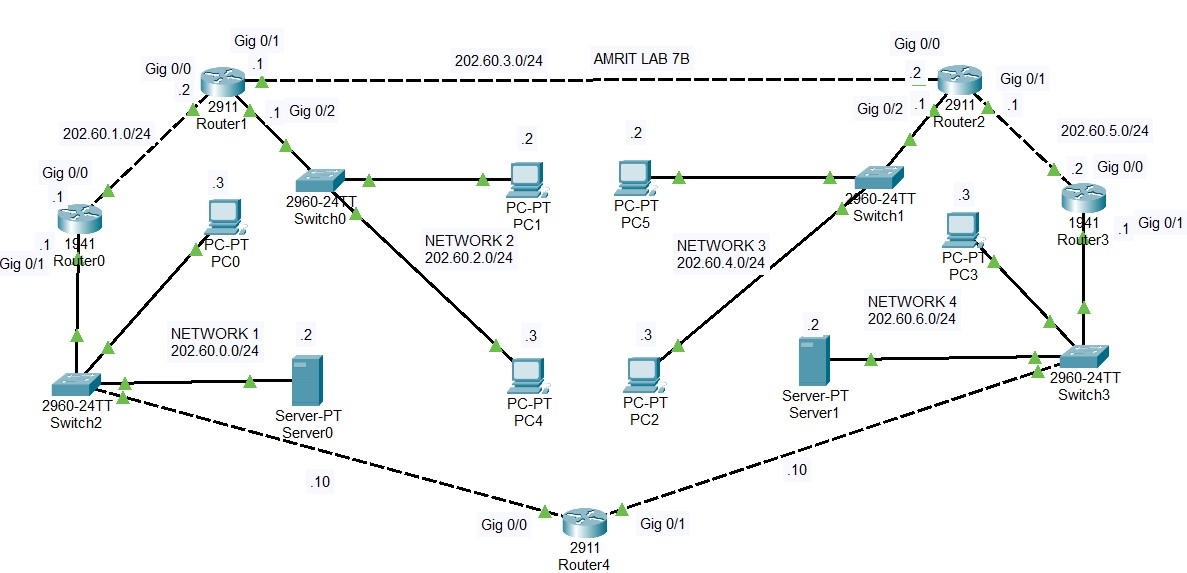
\includegraphics[scale=0.7,cframe=blue 0.5pt 3pt]{./FIG/Lab7B.jpg}
    \caption{Network topology Lab 7B}
\end{figure}

First Disable Passive interface for Network 1 and Network 4 in order to receive updates in Router 4.

\CMD{./CODES/BR4IPR.txt}{Assigning Ip and Configuring RIP Router 4}


\begin{enumerate}

    \item \textbf{Observe the output of show ip route command in each router, and compare with that of
              previous case that is specified in Activity A.}

          \addtocontents{lol}{\protect\subsubsection*{B.1 : \textit{show ip route} in each Router and Compare }}

          \CMD{./CODES/B_Showip0R.txt}{\textit{show ip route} Router 0}
          \CMD{./CODES/B_Showip1R.txt}{\textit{show ip route} Router 1}
          \CMD{./CODES/B_Showip2R.txt}{\textit{show ip route} Router 2}
          \CMD{./CODES/B_Showip3R.txt}{\textit{show ip route} Router 3}
          \CMD{./CODES/B_Showip4R.txt}{\textit{show ip route} Router 4}


          After enabling RIP on additional Router (Router 4) the Routing table in each router has been updated to reach its destination with minimum hops or through shortest path. For example in Router 0, previously there was entry to reach Network 4 through 202.60.1.0 network taking 3 hops but now it has been updated through 200.60.0.10 in 1 hop.


    \item \textbf{Use tracert command from each PC to each another PC and note down the result. Note how
              the changing network topology is addressed by dynamic routing automatically.}

          \addtocontents{lol}{\protect\subsubsection*{B.2 : \textit{tracert} in each Router and Compare }}

          \CMD{./CODES/BT0-1.txt}{Trace Route from PC0 to PC1}
          \CMD{./CODES/BT0-2.txt}{Trace Route from PC0 to PC2}
          \CMD{./CODES/BT0-3.txt}{Trace Route from PC0 to PC3}

          \CMD{./CODES/BT1-2.txt}{Trace Route from PC1 to PC2}
          \CMD{./CODES/BT1-3.txt}{Trace Route from PC1 to PC3}

          \CMD{./CODES/BT2-3.txt}{Trace Route from PC2 to PC3}

          \CMD{./CODES/BT3-4.txt}{Trace Route from PC3 to PC4}
          \CMD{./CODES/BT3-5.txt}{Trace Route from PC3 to PC5}
          \CMD{./CODES/BT3-0.txt}{Trace Route from PC3 to PC0}

          With RIP and Shortest path algorithm Router now has data or routes to reach destination through shortest routes. Taking PC0 and PC3 as example, Before introducing Router 4 between Network 1 and 4 , Packets from PC0 has to travel through Router 1 then Router 2 then Router 3 and finally to PC3 But now Packets can reach to PC3 in 1 hops through Router 4.



    \item \textbf{Now disconnect the link between Router0 and Router1 and observe the output while using
              tracert command from each PC to each another PC. Note how changing network topology
              is addressed in dynamic routing. Also observe the routing table of each router using show
              ip route.}


          \addtocontents{lol}{\protect\subsubsection*{B.3 : Trace Route and Routing Table after diconnecting \textbf{202.60.1.0/24} line}}



          \CMD{./CODES/BT0-1D1.txt}{Trace Route from PC0 to PC1}
          \CMD{./CODES/BT5-0D1.txt}{Trace Route from PC5 to PC0}
          \CMD{./CODES/BT4-0D1.txt}{Trace Route from PC4 to PC0}


          \CMD{./CODES/B_Showip0D1.txt}{\textit{show ip route} Router 0}
          \CMD{./CODES/B_Showip1D1.txt}{\textit{show ip route} Router 1}
          \CMD{./CODES/B_Showip2D1.txt}{\textit{show ip route} Router 2}
          \CMD{./CODES/B_Showip3D1.txt}{\textit{show ip route} Router 3}
          \CMD{./CODES/B_Showip4D1.txt}{\textit{show ip route} Router 4}

          Through \textit{tracert} output of PCs and Routing Table of routers , it is clear that Router has Successfully adapted to change in topology hence determine shortest and alternative Router to destination. For example, Previously Packets from PC4 used to travel  through 202.60.1.0 to Router 0 and then to PC0 but as that link is down Router has determined the alternative path theough Router 2 then Router 3 then Router 4 and finally to PC0.


    \item \textbf{Similarly observe the routing table of each router and output of traceroute/tracert command
              by removing different links between routers as well as by connecting the links.}

          \addtocontents{lol}{\protect\subsubsection*{B.3 : Trace Route and Routing Table after diconnecting \textbf{202.60.3.0/24} line}}

          Trace Route and Routing Table after diconnecting \textbf{202.60.3.0/24} line:

          \CMD{./CODES/BT0-2D3.txt}{Trace Route from PC0 to PC2}
          \CMD{./CODES/BT1-5D3.txt}{Trace Route from PC1 to PC5}
          \CMD{./CODES/BT3-4D3.txt}{Trace Route from PC3 to PC4}


          \CMD{./CODES/B_Showip0D3.txt}{\textit{show ip route} Router 0}
          \CMD{./CODES/B_Showip1D3.txt}{\textit{show ip route} Router 1}
          \CMD{./CODES/B_Showip2D3.txt}{\textit{show ip route} Router 2}
          \CMD{./CODES/B_Showip3D3.txt}{\textit{show ip route} Router 3}
          \CMD{./CODES/B_Showip4D3.txt}{\textit{show ip route} Router 4}

          Here PC1 uses the Routes through PC4 to reach PC2 after link to connect these Network is disconnected.

    \item \textbf{Note down how the changing network topology is addressed by dynamic routing protocol
              automatically to determine the optimal path to reach each of the destination network.}

          Through RIP protocol, Routing information is periodically shared between the routers so, when any changes is detected, it first update its routing table then send updates to neighbors about changes and its available neighbors.






\end{enumerate}

\pagebreak
%%%%%%%%%%%%%%%%%%%%%%%%%%%%%%%%%%%%%%%%%%%%%%%%%%%%%%%%%%%%%%%%%%%
%%%%%%%

%

%

%

%
%%%%%%%%%%%%%%%%CCCCCCCCCCCCCCCCCCCCC
%%%%%%%%%%%%%%%%CCCCCCCCCCCCCCCCCCCCC
%%%%%%%%%%%%%%%%CCCCCCCCCCCCCCCCCCCCC
%%%%%%%%%%%%%%%%CCCCCCCCCCCCCCCCCCCCC
%%%%%%%%%%%%%%%%CCCCCCCCCCCCCCCCCCCCC
%

%

%

%

\addtocontents{lol}{\protect\subsection*{\HRule \\ Activities C\\ \HRule}}

\addtocontents{lof}{\protect\subsection*{\HRule \\ Activities C\\ \HRule}}

\subsubsection{Activities C}

{\bfseries \textit{C. Create the network topology as shown in figure below and perform the following activities:}}


\begin{figure}[H]
    \centering
    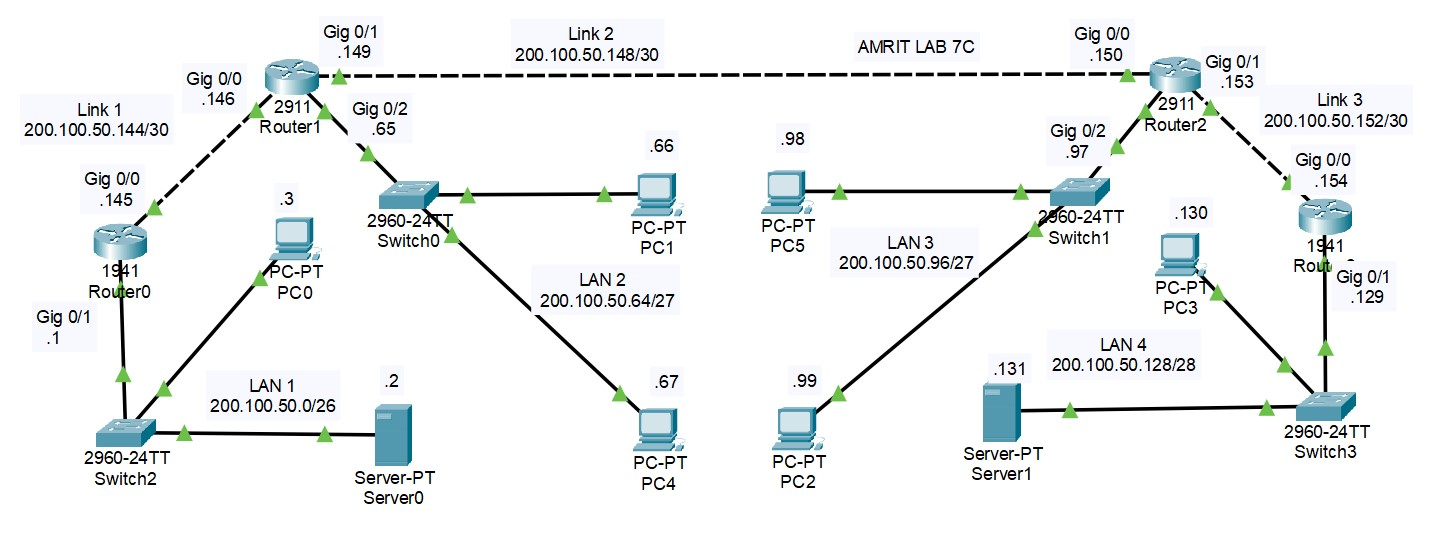
\includegraphics[scale=0.61,cframe=blue 0.5pt 3pt]{./FIG/Lab7C.jpg}
    \caption{Network topology Lab 7C}
\end{figure}
\begin{enumerate}


    \item \textbf{You have given an IP addresses of 200.100.50.0/24. You have to divide this address range
              for different LANs i.e. LAN1, LAN2, LAN3 and LAN4 interconnected as shown in figure
              above, each LAN having 60, 27, 25 and 12 number of hosts. In addition to this there are
              few networks having only two host in each (i.e. connection between two routers). Allocate
              the IP address range for each of the sub-networks with their network address, broadcast
              address and subnet mask. Also list out the unused range of IP addresses (if any)}

          % \usepackage{colortbl}


          \begin{table}[H]
              \centering
              \begin{tabular} {| m{3em} | m{3em} | m{4em} | m{6em} | m{2em} | m{7em} | m{7em} | m{6em} |}
                  \rowcolor[rgb]{0.278,0.573,0.792} \textbf{Subnet Name} & \textbf{Needed Size} & \textbf{Allocated Size} & \textbf{Network Address} & \textbf{Mask} & \textbf{Dec Mask} & \textbf{Assignable Range}       & \textbf{Broadcast Address} \\
                  \hline
                  \textbf{LAN 1}                                         & 60                   & 62                      & 200.100.50.0             & /26           & 255.255.255.192   & 200.100.50.1 - 200.100.50.62    & 200.100.50.63              \\
                  \hline
                  \textbf{LAN 2}                                         & 27                   & 30                      & 200.100.50.64            & /27           & 255.255.255.224   & 200.100.50.65 - 200.100.50.94   & 200.100.50.95              \\
                  \hline
                  \textbf{LAN 3}                                         & 25                   & 30                      & 200.100.50.96            & /27           & 255.255.255.224   & 200.100.50.97 - 200.100.50.126  & 200.100.50.127             \\
                  \hline
                  \textbf{LAN 4}                                         & 12                   & 14                      & 200.100.50.128           & /28           & 255.255.255.240   & 200.100.50.129 - 200.100.50.142 & 200.100.50.143             \\
                  \hline
                  \textbf{Link 1}                                        & 2                    & 2                       & 200.100.50.144           & /30           & 255.255.255.252   & 200.100.50.145 - 200.100.50.146 & 200.100.50.147             \\
                  \hline
                  \textbf{Link 2}                                        & 2                    & 2                       & 200.100.50.148           & /30           & 255.255.255.252   & 200.100.50.149 - 200.100.50.150 & 200.100.50.151             \\
                  \hline
                  \textbf{Link 2}                                        & 2                    & 2                       & 200.100.50.152           & /30           & 255.255.255.252   & 200.100.50.153 - 200.100.50.154 & 200.100.50.155             \\
                  \hline
              \end{tabular}
              \caption{Assignning IP thropugh VLSM}
          \end{table}


          The unused IP range is \textbf{ 200.100.50.156 - 200.100.50.255}


    \item \textbf{On the basis of your division configure IP address for each interface of routers. Also configure the IP address and default gateway of each PC and server.}

          \addtocontents{lol}{\protect\subsubsection*{C.2 : Configure IP  in Router and PCs}}

          \CMD{./CODES/C_ConfigR0.txt}{Configure Router 0}

          \CMD{./CODES/C_ConfigR1.txt}{Configure Router 1}

          \CMD{./CODES/C_ConfigR2.txt}{Configure Router 2}

          \CMD{./CODES/C_ConfigR3.txt}{Configure Router 3}



          \begin{figure}[H]
              \centering
              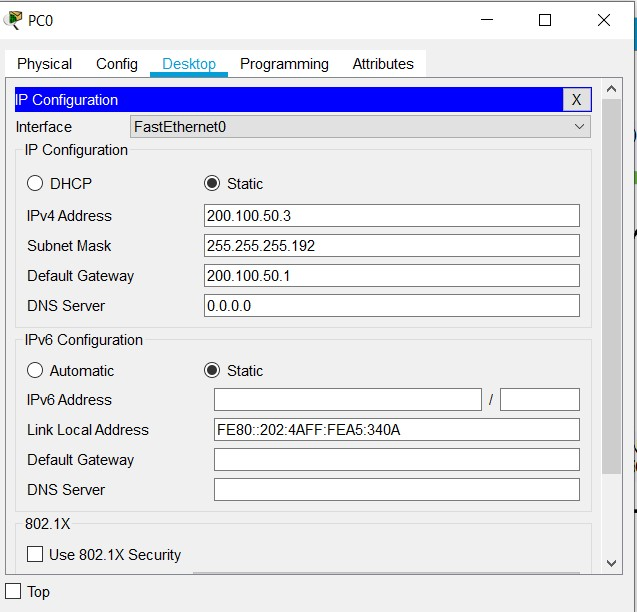
\includegraphics[scale=0.81,cframe=blue 0.5pt 3pt]{./FIG/CPC0.jpg}
              \caption{Config IP and Default gateway in PC 0}
          \end{figure}

          \begin{figure}[H]
              \centering
              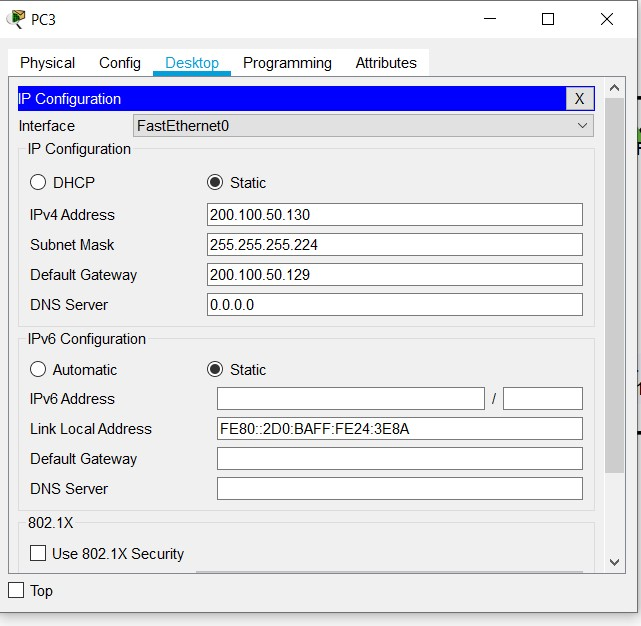
\includegraphics[scale=0.81,cframe=blue 0.5pt 3pt]{./FIG/CPC3.jpg}
              \caption{Config IP and Default gateway in PC 3}
          \end{figure}


          \begin{figure}[H]
              \centering
              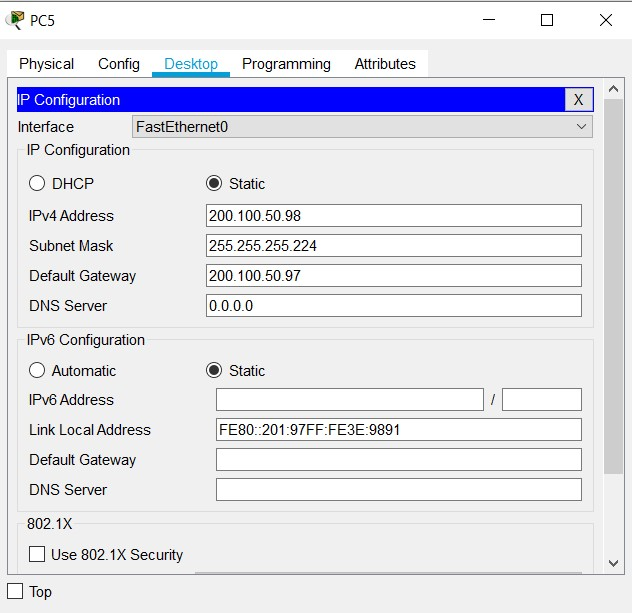
\includegraphics[scale=0.81,cframe=blue 0.5pt 3pt]{./FIG/CPC5.jpg}
              \caption{Config IP and Default gateway in PC 5}
          \end{figure}


    \item \textbf{Enable routing in between LANs using OSPF. Test the connectivity from a pc of any LAN
              to pc of any another LAN by using ping.}



          \addtocontents{lol}{\protect\subsubsection*{C.3 : Enable Routing using OSPF and Testing}}

          \CMD{./CODES/C_RouteR0.txt}{Routing using OSPF Router 0}

          \CMD{./CODES/C_RouteR1.txt}{Routing using OSPF Router 1}

          \CMD{./CODES/C_RouteR2.txt}{Routing using OSPF Router 2}

          \CMD{./CODES/C_RouteR3.txt}{Routing using OSPF Router 3}





          \CMD{./CODES/CP0-1.txt}{Ping from PC0 to PC1}
          \CMD{./CODES/CP1-2.txt}{Ping from PC1 to PC2}
          \CMD{./CODES/CP2-3.txt}{Ping from PC2 to PC3}
          \CMD{./CODES/CP0-2.txt}{Ping from PC0 to PC2}
          \CMD{./CODES/CP3-1.txt}{Ping from PC3 to PC1}
          \CMD{./CODES/CP3-0.txt}{Ping from PC3 to PC0}

          All Ping are Successful after using OSPF routing Protocols. Similar to RIP , OSPF also adapts the Routing table as per the changes im its Topology and has initials as \textbf{O} in its Routing Table.



    \item \textbf{Note down the result of traceroute using traceroute command from PC0 to PC3}

          \addtocontents{lol}{\protect\subsubsection*{C.4 : Trace Route from PC0 to PC3}}

          \CMD{./CODES/CT0-3.txt}{Trace Route from PC0 to PC3}



    \item \textbf{Observe the routing table in each router by using show ip route command.}

          \addtocontents{lol}{\protect\subsubsection*{C.5 : Routing Table}}

          \CMD{./CODES/C_Showip0.txt}{\textit{show ip route} Router 0}
          \CMD{./CODES/C_Showip1.txt}{\textit{show ip route} Router 1}
          \CMD{./CODES/C_Showip2.txt}{\textit{show ip route} Router 2}
          \CMD{./CODES/C_Showip3.txt}{\textit{show ip route} Router 3}

\end{enumerate}

\pagebreak

%%%%%%%%%%%%%%%%%%%%%%%%%%%%%%%%%%%%%%%%%%%%%%%%%%%%%%%%%%%%%%%%

%
%
%
%

%5%%%%%%%%%%%%%%%%%%%%DDDDDDDDDDDDDDDDDDDD
%5%%%%%%%%%%%%%%%%%%%%DDDDDDDDDDDDDDDDDDDD
%5%%%%%%%%%%%%%%%%%%%%DDDDDDDDDDDDDDDDDDDD
%5%%%%%%%%%%%%%%%%%%%%DDDDDDDDDDDDDDDDDDDD
%5%%%%%%%%%%%%%%%%%%%%DDDDDDDDDDDDDDDDDDDD
%
%
%
%
%
%
%

\addtocontents{lol}{\protect\subsection*{\HRule \\ Activities D\\ \HRule}}

\addtocontents{lof}{\protect\subsection*{\HRule \\ Activities D\\ \HRule}}

\subsubsection{Activities D}

{\bfseries \textit{D.Now Connect additional router as shown in figure below:}}



\begin{figure}[H]
    \centering
    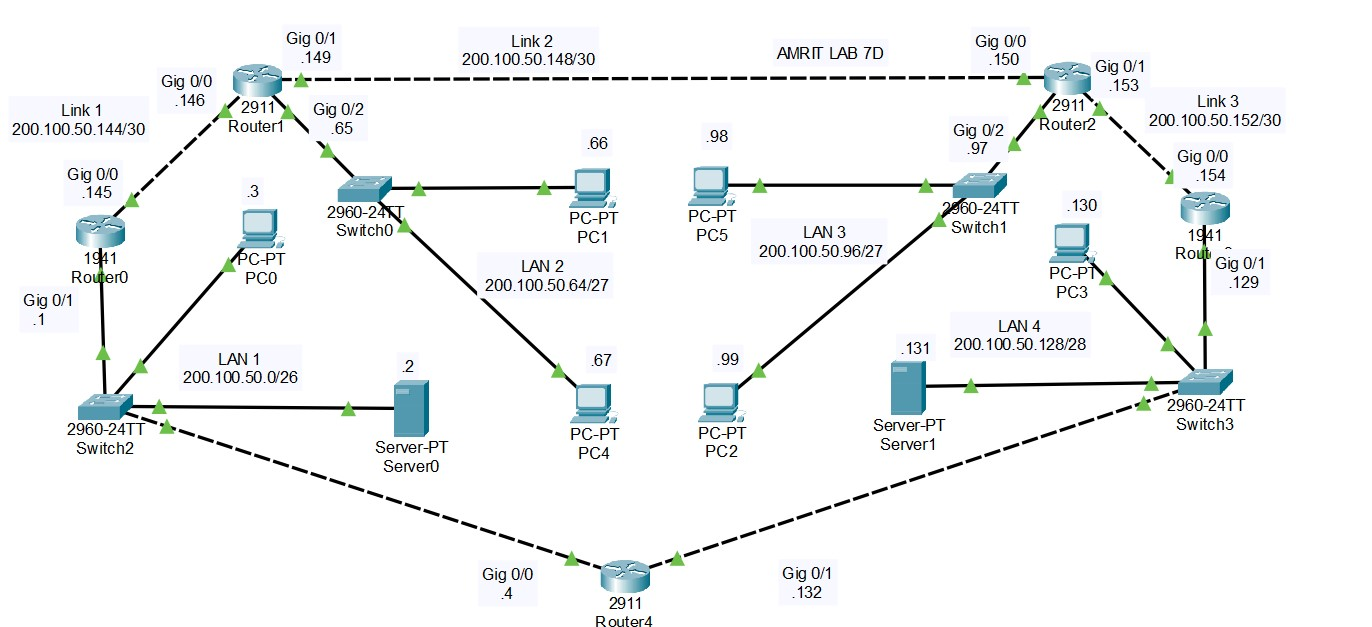
\includegraphics[scale=0.62,cframe=blue 0.5pt 3pt]{./FIG/Lab7D.jpg}
    \caption{Network topology Lab 7D}
\end{figure}



\begin{enumerate}

    \item \textbf{Configure the interfaces of Router4 with appropriate IP addresses and enable OSPF in it.
              Now note down the result of traceroute command from PC3 to PC0 and routing table in
              each router. Compare the result of previous.}


          \addtocontents{lol}{\protect\subsubsection*{D.1 : Configure IP and Enable OSPF in Router 0}}

          \CMD{./CODES/D_ConfigR4.txt}{Configure Router 4}


          \CMD{./CODES/D_RouteR4.txt}{Routing using OSPF Router 4}



          \CMD{./CODES/DT3-0.txt}{Trace Route from PC3 to PC0}



          \CMD{./CODES/D_Showip0.txt}{\textit{show ip route} Router 0}
          \CMD{./CODES/D_Showip1.txt}{\textit{show ip route} Router 1}
          \CMD{./CODES/D_Showip2.txt}{\textit{show ip route} Router 2}
          \CMD{./CODES/D_Showip3.txt}{\textit{show ip route} Router 3}
          \CMD{./CODES/D_Showip4.txt}{\textit{show ip route} Router 4}

          With addition of Router 4 there is noticeable changes in Routing Tables in all Routers.
          From above Trace route and Routing table of Router 3 one can explain how OSPF adapts to changes and determine the shortest path to destination.


    \item \textbf{Remove a link i.e. the link between router 4 and switch 0 and then observe the result of
              traceroute command from PC3 to PC0 and routing table in each router. Compare the result
              of previous. Note down how the routing is updated to address the changing topology.}


          \addtocontents{lol}{\protect\subsubsection*{D.2 : Removing Link and observing Route path amd Routing table}}

          The link between Router 4 and switch 2 of LAN 1(200.100.50.0/26) is removed.


          \CMD{./CODES/DT3-0D1.txt}{Trace Route from PC3 to PC0}

          \CMD{./CODES/D_Showip0D1.txt}{\textit{show ip route} Router 0}
          \CMD{./CODES/D_Showip1D1.txt}{\textit{show ip route} Router 1}
          \CMD{./CODES/D_Showip2D1.txt}{\textit{show ip route} Router 2}
          \CMD{./CODES/D_Showip3D1.txt}{\textit{show ip route} Router 3}
          \CMD{./CODES/D_Showip4D1.txt}{\textit{show ip route} Router 4}



    \item \textbf{Again connect the link and repeat the observations.}

          Observation is Similar to Activity D.1 that is before  disconnection.


    \item \textbf{You can observe by removing another link between Router0 and Router1 also.}
          \addtocontents{lol}{\protect\subsubsection*{D.4 : Removing Link 1 and observing Route path amd Routing table}}

          After removing Link 1 (200.100.50.144/30) following Observation is done.

          \CMD{./CODES/DT1-0L1.txt}{Trace Route from PC1 to PC0}

          \CMD{./CODES/D_Showip0L1.txt}{\textit{show ip route} Router 0}
          \CMD{./CODES/D_Showip1L1.txt}{\textit{show ip route} Router 1}
          \CMD{./CODES/D_Showip2L1.txt}{\textit{show ip route} Router 2}
          \CMD{./CODES/D_Showip3L1.txt}{\textit{show ip route} Router 3}
          \CMD{./CODES/D_Showip4L1.txt}{\textit{show ip route} Router 4}




    \item \textbf{Similarly you can observe by removing other links.}

          \addtocontents{lol}{\protect\subsubsection*{D.4 : Removing Link 2 and observing Route path amd Routing table}}

          After removing Link 1 (200.100.50.148/30) following Observation is done.


          \CMD{./CODES/DT1-2L2.txt}{Trace Route from PC1 to PC2}

          \CMD{./CODES/D_Showip0L2.txt}{\textit{show ip route} Router 0}
          \CMD{./CODES/D_Showip1L2.txt}{\textit{show ip route} Router 1}
          \CMD{./CODES/D_Showip2L2.txt}{\textit{show ip route} Router 2}
          \CMD{./CODES/D_Showip3L2.txt}{\textit{show ip route} Router 3}
          \CMD{./CODES/D_Showip4L2.txt}{\textit{show ip route} Router 4}


\end{enumerate}






%%%%%%%%%%%%%%%%%%%%%%%%%%%%%%%%%%%%%%%%%%%%%%%%%%%%%%%%%%%%%%%%%%%%%%%%%%%

%%%%%%%%%%%%%%%%%%%%%%%%%%%%4444444444444444444444444444444444
\begin{Q}
    {
        How dynamic routing can address the changing topology of a network automatically?
        Explain with reference to the observation of your lab exercise.
    }
\end{Q}

\begin{A}
    {
        Dynamic Routing is Adaptive routing technique. Here in this LAb we explore RIp and OSPF . In dynamic Routing, Routers shares the routing Information to its Neighbors and neighbor updates its routing table if any shortest path to any network is found.

        RIP uses distance vector algorithm where as OSPF Dijkstra’s algorithm to determine the shortest path to destination.
    }
\end{A}


%%%%%%%%%%%%%%%%%%%%%%%%%%%%%%%%%%%%%%%%%%%%%%%%%%%%%%%%%%%%%%%%%%%%%%%%%%%




\section{Conclusion}

In this Lab we familiarize ourselves with dynamic Routing and its protocols like RIP and OSPF.
In Activity A we created the setup and Configured RIP and tested with the help of Ping and Tracert command. In Activity B we connected additional router and studied the changes it makes to the routing tables. We also observe the output after disconnecting different links and how Network reacts and stay connected during that time. Activity C and D are based on OSPF with additional touch of VLSM .


\end{document}